\chapter{Elastic rod : equilibrium approach}

\section{Introduction}
Ici on explique que l'approche par les équations d'équilibre est beaucoup plus directe que l'approche énergétique.

\subsection{Goals and contribution}
Dans ce chapitre, après un bref rappel sur le cadre mathématique d'étude des courbes paramétrique de l'espace, on présente les notions de courbures et de torsion géométrique associées au repère de fraient. On montre ensuite le cas plus général d'un repère mobile quelconque attaché à une courbe gamma. On définit enfin la particularité d'un repère mobile adapté à un courbe, et on présente, en sus du repère de Frenet, une approche différente pour accrocher des repères le long d'une courbe (Bishop / RMF / Zéro-twisting frame)

Ici il faudrait préciser la terminologie des auteurs / équations / hypothèses :
Euler-Bernoulli, Navier-Bernoulli, Kirchhoff, Love, Clebesh, Cosserat, Vlassov

\subsection{Related work}
On peu s'instruire dans la publi de Dill \cite{Dill1992}.
Regarder en particulier le premier chapitre de l'HDR de Neukirch \cite{Neukirch2009}.
Regarder également la chronologie des modèles proposée dans la thèse de Theetten \cite{Theetten2007}.
Pourquoi pas proposer une frise chronologique + un tableau de synthèse des hyptohèses.

\cite{Dill1992}
\citet{Neukirch2009}
\cite{Adriaenssens1999}
\cite{Hoogenboom2006}
\cite{Lang2009}
\cite{Spillmann2008}
\cite{Antman2005}

\cite{Neukirch2009} : p69 - \cite{Dill1992} : p16

Dans les tentatives dans notre domaine, citer :

Kirchhoff : \cite{Kirchhoff1850, Kirchhoff1876} \\
Clebsch : \cite{Clebsch1883} \\
Love : \cite{Love1892} \\
Timoshenko : \cite{Timoshenko1921, Timoshenko1922, Timoshenko1951}

\blockcquote[p.~607]{Langer1996}{Note that $\gamma$ having unit speed corresponds to the rod being inextensible; this is not always assumed in the theory, nor is the material frame necessarily assumed to be orthonormal as it is here}

\blockcquote[p.~607]{Langer1996}{Natural frames and the curve angle representation of rod}


Départ :
\cite{Day1965} : already includes a rotational DOF !!
\cite{Wakefield1980}
\cite{Barnes1999} : revue intéressante de la DR.

3 pts classique :
\cite{Adriaenssens1999}
\cite{Douthe2006}

2 x 3pts :
\cite{Barnes2013}

6 Dofs :
\cite{DAmico2014}

4Dofs :
\cite{DuPeloux2015}
\cite{DAmico2016}

Dans le champ de l'animation  avec élément finis
\cite{Duan2013}
\cite{Meier2014}


\subsection{Overview}
Résumé du chapitre

\footnote{For a shearable rod, the condition that $\vect{d}_3$ and $\vect{t}$ coincide is relaxed.}
\footnote{in the directions of the principal axes of inertia of its cross-section}
\footnote{The parameter $\rconf{s}$, usually chosen as the arc length parameter for the undeformed rod, is no longer the arc length parameter for the deformed rod, since there are deformations of shear and extension. The current arc length of the deformed rod is a function of $\rconf{s}$, which is often denoted by $s(\rconf{s})$.}


\blockcquote[p.~xvii]{Benvenuto1991b}{The battle between weight and rigidity constitutes, in itself, the single aesthetic theme of art in architecture : and to bring out this conflict in the most varied and clearest way is its office.}

\blockcquote[p.~xvii]{Villaggio1997}{The theory of elastic structures is, by definition, the collection of all reasonable models, proposed during almost three centuries, concerned with simplifying the solutions of problems involving elastic bodies. The equations describing the motion and equilibrium of a three-dimensional elastic body were formulated in full generality during the first half of the nineteenth century, but their solutions are known only in a few cases.}

\blockcquote[p.~68]{Audoly2010}{In a deformed state, the center line has no particular reason to remain straight and, in general, $\vect{d}_1$ and $\vect{d}_2$ will twist along the center line. However, in the case of small strain that we consider, the triad $(\vect{d}_1,\vect{d}_2,\vect{d}_3)$ remains approximately orthonormal, provided it has been chosen orthonormal in the reference configuration. This is known as the Euler-Bernoulli or Navier-Bernoulli kinematical hypothesis, or sometimes the assumption of unshearable rods.}

Extension to the case of thin-walled sections by \cite{Dias2015, Vetyukov2014} in the case of ribbons. From the Vlasov

\blockcquote[p.]{Dias2014}{For thin beams having a slender cross-section, $h \ll w$, the classical rod theory of Kirchhoff is known to be inapplicable. Such beams are usually modeled using Vlasov’s theory for thin-walled beams. Vlasov’s models can be justified from 3D elasticity but only in the case of moderate deformations, when the cross-sections bend by a small amount. In the present work, however, we have considered large deformations of thin strips. The strip has been modeled as an inextensible  plate, and the geometric  constraint of inextensibility has been treated exactly : the cross-sections are allowed to bend by a significant amount. Our model extends the classical strip model of Sadowsky, and reformulate it in a way that fits into the classical theory of rods.}

\clearpage
\section{Introduction to the special Cosserat theory of rods}

This paragraph gives a (very) brief overview of the \emph{special Cosserat theory of rods}, as presented in \cite{Antman2005}, that accounts for bending, torsion, extension and shear  behaviors of slender beams.\footnote{\blockcquote[p.~270]{Antman2005}{[we formulate] a general dynamical theory of rods that can undergo large deformations in space by suffering flexure, torsion, extension, and shear. We call the resulting geometrically exact theory the \emph{special Cosserat theory of rods}.}} It gives a larger scope to the basements of the present work -- which relies on the \emph{Kirchhoff theory of rods} -- as the last is a special case of this larger theoretical framework. Thus, what is presented in this paragraph could be considered as a reasonable starting point to extend the present work, for instance to take account for shear or large extension, which might be relevant for some engineering problems or form-finding processes.

This theory was introduce by \cite{Antman1974}. It has been largely employed in various fields \cite{Shi1995, Bergou2010}.

%\begin{figure}[p]
%  	\begin{leftfullpage}
%		\captionsetup[subfloat]{captionskip=10pt}
%     		\centering
%     		\subfloat[][]{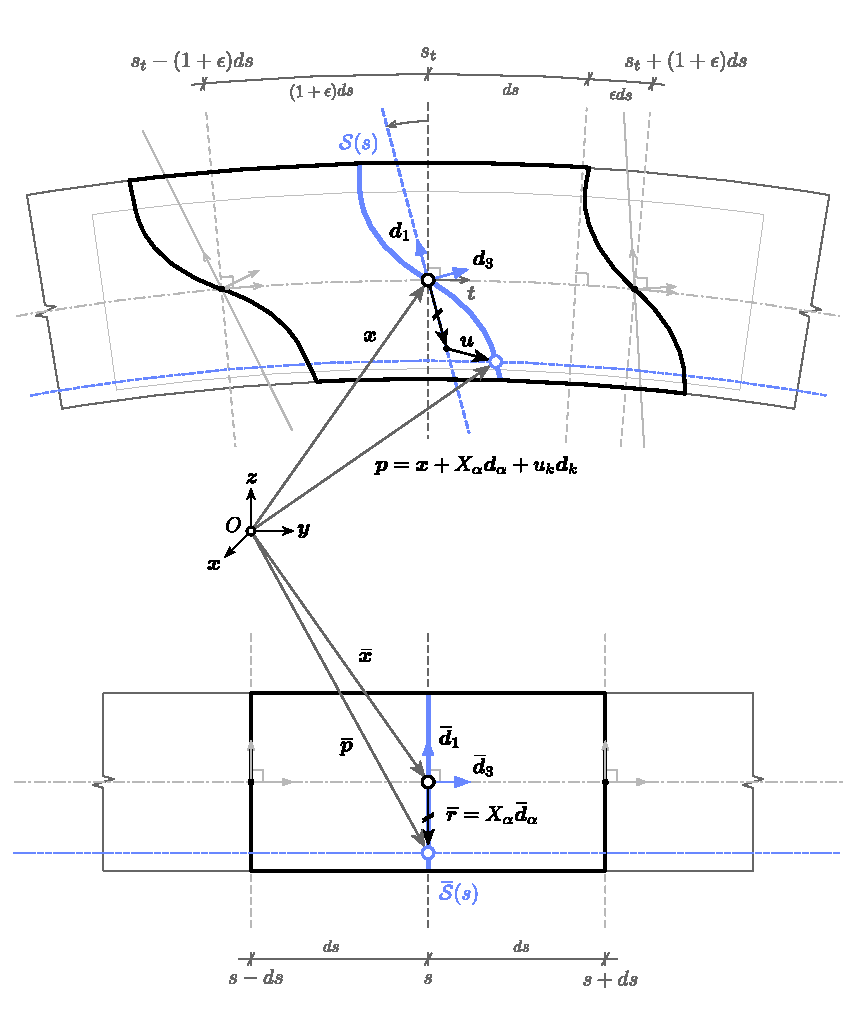
\includegraphics{cosserat_motion_longi.pdf}\label{fig:cosserat_1}}
%		\caption{Description of the motion for a Cosserat rod. This is a typical longitudinal section of a rectangular beam deformed from a reference configuration (bottom) to an actual configuration (top). Cross-sections are defined in the reference configuration to be planar surfaces perpendicular to the beam axis. A material point $\rconf{\vect{p}} \in \rconf{\mathcal{S}}(s)$ is located relatively to the cross-section centroid ($\rconf{\vect{x}}$) thanks to its material coordinates ($X_1$, $X_2$). During the motion, this material point reach a new position $\vect{p} \in \mathcal{S}(s)$. The deformed cross-section is no more planar. The material frame is no more aligned with the beam axis ($\vect{d}_3$ and $\vect{t}$ are not parallel any more). The actual position is measured from the centroid of the deformed cross-section ($\rconf{\vect{x}}$) plus an in-plane component ($X_{\alpha}\vect{d}_{\alpha}$) and a deformation vector ($\vect{u}$). If the cross-sections deform in a rigid-body manner, then $\vect{u}$ is null everywhere.}
%	 \end{leftfullpage}
%\end{figure}
%\begin{figure}[p]
%	\begin{fullpage}
%		\captionsetup[subfloat]{captionskip=10pt}
%     		\centering
%     		\subfloat[][Cross-section $\mathcal{S}(s)$.]{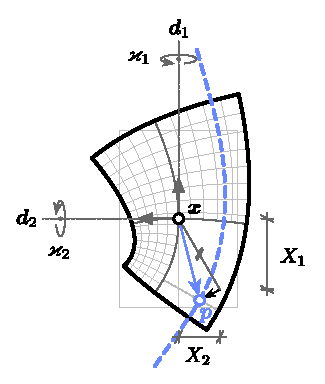
\includegraphics{cosserat_motion_trans_def_a.pdf}\label{fig:cosserat_2a}}
%		\subfloat[][Cross-section $\mathcal{S}(s+ds)$.]{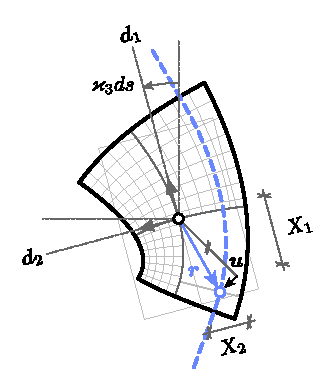
\includegraphics{cosserat_motion_trans_def_b.pdf}\label{fig:cosserat_2b}} \\
%%		\vspace{30pt}
%		\subfloat[][Cross-section $\rconf{\mathcal{S}}(s)$.]{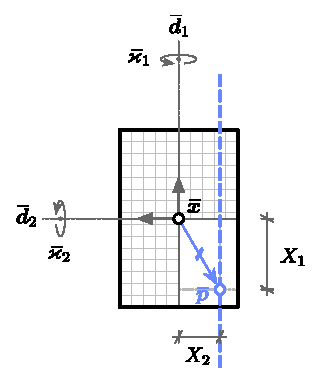
\includegraphics{cosserat_motion_trans_ref_a.pdf}\label{fig:cosserat_2c}}
%		\subfloat[][Cross-section $\rconf{\mathcal{S}}(s+ds)$.]{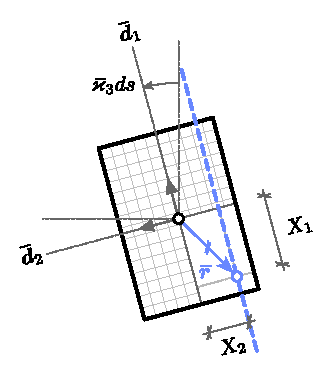
\includegraphics{cosserat_motion_trans_ref_b.pdf}\label{fig:cosserat_2d}}
%%		\vspace{30pt}
%		\label{fig:cosserat_2}
%		\caption{Description of the motion for a Cosserat rod. These are the transversal sections from \cref{fig:cosserat_1}. Remark how the deformed material point is located through $\vect{x}$ and $\vect{r} = X_{\alpha}\vect{d}_{\alpha} + u_{k}\vect{d}_{k}$. Cross-sections are rotating around $\vect{d}_3$ at speed $\varkappa_3$.}    
%	\end{fullpage}
%\end{figure}


\begin{figure}[p]
  	\begin{leftfullpage}
		\centering
     		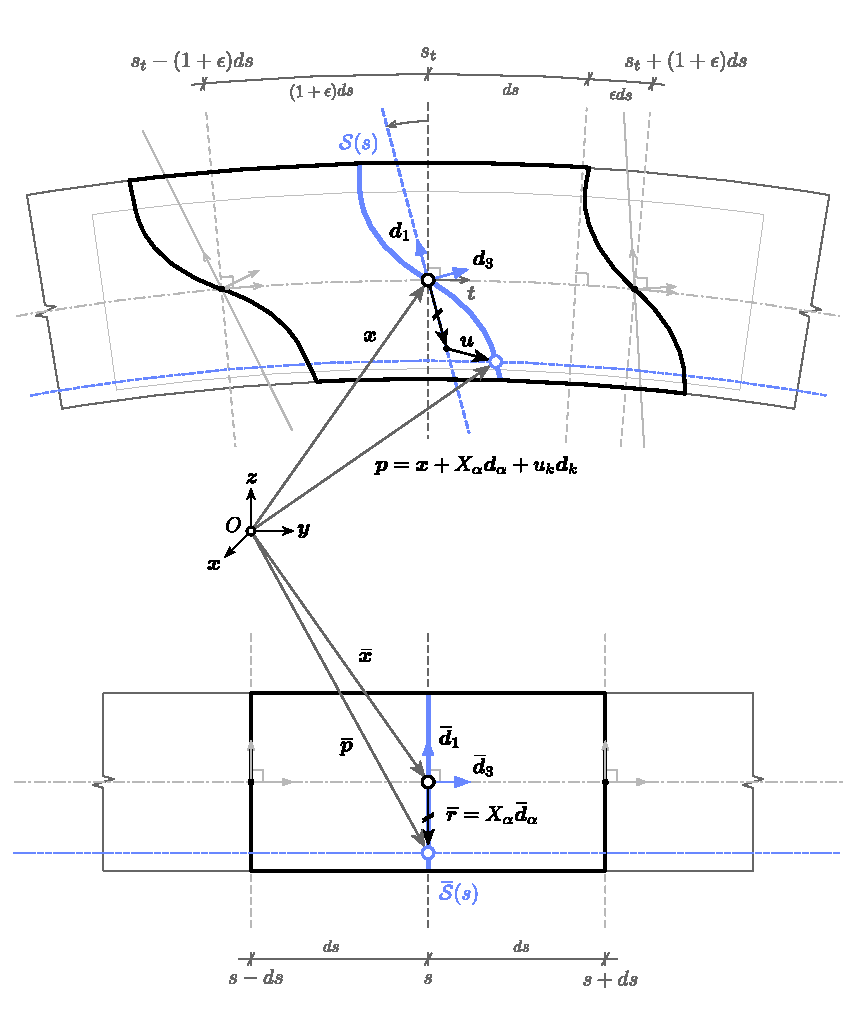
\includegraphics{cosserat_motion_longi.pdf}
		\caption{Description of the motion for a Cosserat rod. This is a typical longitudinal section of a rectangular beam deformed from a reference configuration (bottom) to an actual configuration (top). Cross-sections are defined in the reference configuration to be planar surfaces perpendicular to the beam axis. A material point $\rconf{\vect{p}} \in \rconf{\mathcal{S}}(s)$ is located relatively to the cross-section centroid ($\rconf{\vect{x}}$) thanks to its material coordinates ($X_1$, $X_2$). During the motion, this material point reach a new position $\vect{p} \in \mathcal{S}(s)$. The deformed cross-section is no more planar. The material frame is no more aligned with the beam axis ($\vect{d}_3$ and $\vect{t}$ are not parallel any more). The actual position is measured from the centroid of the deformed cross-section ($\rconf{\vect{x}}$) plus an in-plane component ($X_{\alpha}\vect{d}_{\alpha}$) and a deformation vector ($\vect{u}$). If the cross-sections deform in a rigid-body manner, then $\vect{u}$ is null everywhere.}
		\label{fig:cosserat_1}
	 \end{leftfullpage}
\end{figure}
\begin{figure}[p]
	\begin{fullpage}
		\captionsetup[subfloat]{captionskip=10pt}
     		\centering
     		\subfloat[][Deformed cross-section $\mathcal{S}(s)$.]{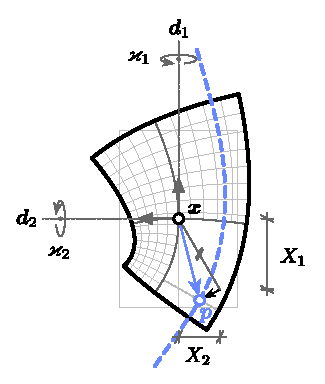
\includegraphics{cosserat_motion_trans_def_a.pdf}\label{fig:cosserat_2a}}
		\hspace{2.5cm}
		\subfloat[][Deformed cross-section $\mathcal{S}(s+ds)$.]{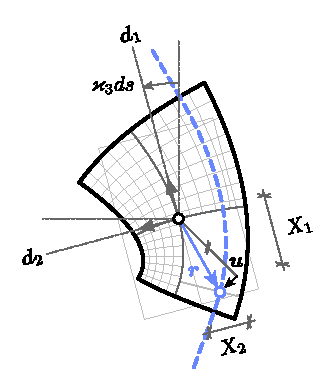
\includegraphics{cosserat_motion_trans_def_b.pdf}\label{fig:cosserat_2b}} \\
		\vspace{20pt}
		\subfloat[][Reference cross-section $\rconf{\mathcal{S}}(s)$.]{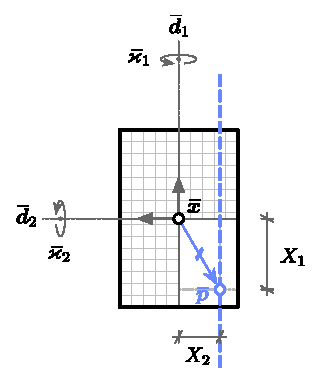
\includegraphics{cosserat_motion_trans_ref_a.pdf}\label{fig:cosserat_2c}}
		\hspace{2.5cm}
		\subfloat[][Reference cross-section $\rconf{\mathcal{S}}(s+ds)$.]{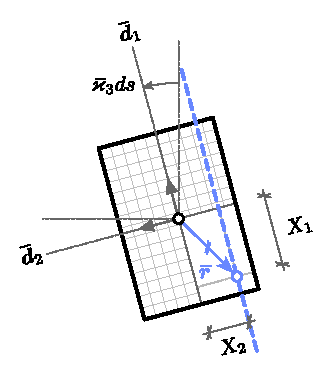
\includegraphics{cosserat_motion_trans_ref_b.pdf}\label{fig:cosserat_2d}}
		\vspace{20pt}
		\caption{Description of the motion for a Cosserat rod. These are the transversal sections from \cref{fig:cosserat_1} -- however note that \cref{fig:cosserat_1} is drawn with $\varkappa_2 < 0$ while $\varkappa_2 > 0$ in \cref{fig:cosserat_2}. The section curve is drawn in a dashed blue fashion. Remark how the deformed material point is located through $\vect{x}$ and $\vect{r} = X_{\alpha}\vect{d}_{\alpha} + u_{k}\vect{d}_{k}$. Cross-sections are rotating around $\vect{d}_3$ at speed $\varkappa_3$. The beam is subject to flexion ($\varkappa_1 > 0$, $\varkappa_2 > 0$), torsion ($\varkappa_3 > 0$) and extension ($\epsilon > 0$). Fibers that are compressed are subjected to transverse expansion due to the Poisson effect (see up-right of \cref{fig:cosserat_2a,fig:cosserat_2b}). Reciprocally, fibers in tension are subjected to transverse contraction (see bottom-left of \cref{fig:cosserat_2a,fig:cosserat_2b}).}
		\label{fig:cosserat_2}    
	\end{fullpage}
\end{figure}

\subsection{Description of the motion}

\cref{fig:cosserat_1}
\cref{fig:cosserat_2}

\begin{table}[p]
\center
	\renewcommand{\arraystretch}{1.8}
	\begin{tabular}{l|c|c} 
		 				& reference configuration										& actual configuration
		\\ \hline
		arc length 			& $s = \Psi_t^{-1}(s_t)$ 										& $s_t = \Psi_t(s)$
		\\ \hline
		length 			& $L$ 													& $L_t$
		\\ \hline
		centerline			& $\gamma$ 												& $\gamma_t$
		\\ \hline
		position vector		& $\rconf{\vect{x}}$ 										& ${\vect{x}}$
		\\ \hline
		material frame		& $\{\rconf{\vect{d}_1},\rconf{\vect{d}_2},\rconf{\vect{d}_3}\}$ 		& $\{\vect{d}_1,\vect{d}_2,\vect{d}_3\}$
		\\ \hline
		force strains 		& $\rconf{\vect{\nu}}$ 										& ${\vect{\nu}}$ 	
		\\ \hline
		moment strains 	& $\rconf{\vect{\varkappa}}$ 									& ${\vect{\varkappa}}$
		\\ \hline
		spin vector 		& $\rconf{\vect{\omega}}$ 									& ${\vect{\omega}}$ 
		\\ \hline
		axial extension 		& $ \rconf{\epsilon} = 0$ 									& $\nu_3 = 1 + \epsilon = \Psi'_t(s)$		
		\\ \hline
		arc length derivative 	& $ \frac{\partial}{\partial s} \cdot = (\cdot)'	$						& $\frac{\partial}{\partial s_t} \cdot = (1 + \epsilon)^{-1} (\cdot)'$			
		\\ \hline
		time derivative 		& $ \frac{\partial}{\partial t} \cdot = \dot{(\cdot)}$						& $ \frac{\partial}{\partial t} \cdot = \dot{(\cdot)}$		
		\\ \hline	
	\end{tabular}
	\label{tab:count}
	\caption{Summary of the notations employed through out this chapter.}
\end{table}

\subsubsection{Actual configuration}

At time $t$, the \emph{actual} or \emph{deformed} configuration of the rod $\{{\vect{x}}, {\vect{d}_1}, {\vect{d}_2}\}$ is described by its \emph{centerline} $\gamma \in \mathcal{C}^1([0,{L}]\times \mathbb{R}^3)$, a regular space curve, 
\begin{equation}
	\fonctionL{\gamma(t, \cdot)}{[0,\rconf{L}]}{\mathbb{R}^3}{\rconf{s}}{\vect{x}(t,\rconf{s})}
\end{equation}
and two perpendicular unit vector fields : 
\begin{equation}
	\fonctionL{(\vect{d}_1,\vect{d}_2)(t, \cdot)}{[0,\rconf{L}]}{\mathbb{R}^3 \times \mathbb{R}^3}{\rconf{s}}{(\vect{d}_1(t,\rconf{s}), \vect{d}_2(t,\rconf{s})) \; / \; 
	\vect{d}_1(t,\rconf{s}) \cdot \vect{d}_2(t,\rconf{s}) = 0
	}
\end{equation}
In addition, we define a third unit vector field as : 
\begin{equation}
	\vect{d}_3 = \vect{d}_1 \times \vect{d}_2
\end{equation}
Thus, the centerline is framed with the orthonormal moving frame $\{\vect{d}_1, \vect{d}_2, \vect{d}_3\}$. The unit vectors $\vect{d}_i(t,\rconf{s})$ are called \emph{material directors}.

Note that the centerline is parametrized by $\rconf{s}$ which is chosen to be the arc length parameter of the \emph{reference} configuration. It may not coincide with the arc length parameter of the \emph{actual} configuration denoted by $s = s(t, \rconf{s})$ as the rod may suffer elongation.

\subsubsection{Reference configuration}
We now identify a \emph{reference} configuration $\{\rconf{\vect{x}}, \rconf{\vect{d}_1}, \rconf{\vect{d}_2}\}$ of the rod as a stress-free configuration when no external loads are applied to the rod. With no loss of generality, this configuration is assumed to be the configuration at time $t=0$. 

In this configuration, the rod is assumed to be prismatic. The centerline is chosen to be the curve passing through the cross-section centroids. We call $\rconf{s}$ its arc length parameter and $\rconf{L}$ its length. The set of rod material points that belong to the plane perpendicular to the centerline at arc length $\rconf{s}$ is classically called a \emph{cross-section}. Note that while cross-sections are defined in the \emph{reference} configuration and are planar by definition, there is no reason that this surface stays planar in any other configuration \cite[p.~5]{Dill1992}.

\subsection{Strains}

We decompose the rod deformations in the material frame basis of the \emph{actual} configuration at position $\rconf{s}$ of the \emph{reference} configuration $\{\vect{d}_1, \vect{d}_2, \vect{d}_3\}(\rconf{s})$.

The deformation of the centerline regarding the variable $\rconf{s}$ is described with the help of the strain vector $\vect{\nu}$ with coordinates $(\nu_1, \nu_2, \nu_3 = 1 + \epsilon)^T$ in the material frame basis : \footnote{The elongation strain is defined in \cite[pp.~283]{Antman2005} as : $\nu_3 = \vect{x}' \cdot (\vect{d}_1 \times \vect{d}_2) =  \vect{x}' \cdot \vect{d}_3 = 1+\epsilon$. $\nu_1$ and $\nu_2$ are called shear strains.}
\begin{equation}
		\frac{\partial \vect{x}}{\partial \rconf{s}} (t, \rconf{s})  = {\nu_1}(t, \rconf{s}) \vect{d}_1(t, \rconf{s})
		+ {\nu_2}(t, \rconf{s}) \vect{d}_2(t, \rconf{s})
		+ {\nu_3}(t, \rconf{s}) \vect{d}_3(t, \rconf{s})
\end{equation}
The deformation of the material frame regarding the variable $\rconf{s}$ is described with the help of the strain vector $\vect{\omega}$ with coordinates $(\kappa_1, \kappa_2, \tau)^T$ in the material frame basis :
\begin{equation}	
		\frac{\partial \vect{d}_i}{\partial \rconf{s}} (t, \rconf{s}) = \vect{\omega}(t, \rconf{s}) \times  \vect{d}_i (t, \rconf{s})
\end{equation}
The velocity of the material frame is described with the help of the spin vector $\vect{w}$ with coordinates $(w_1, w_2, w_3)^T$ in the material frame basis :
\begin{equation}	
		\frac{\partial \vect{d}_i}{\partial t} (t, \rconf{s}) = \vect{w}(t, \rconf{s}) \times  \vect{d}_i (t, \rconf{s})
\end{equation}
Now, the spatial derivative regarding $\rconf{s}$ will be denoted by a prime (${}'$) and the time derivative regardin $t$ by a dot ($\dot{}$).

\subsubsection{Parametrization}

Because the centerline of the reference configuration is parametrized by arc length, the unit tangent vector is given by :
\begin{equation}	
	\rconf{\vect{t}}(t, \rconf{s}) = \frac{\partial \rconf{\vect{x}}}{\partial \rconf{s}} (t, \rconf{s}) = \rconf{\vect{x}}'(t, \rconf{s})
	\quad , \quad
	\norm{\rconf{\vect{x}}'} = 1
\end{equation}
In the deformed configuration, the centerline is still parametrized by $\rconf{s}$ which is no more an arc length parameter as extension happened. Thus, the unit tangent vector is given by :
\begin{equation}	
	\vect{t}(t, \rconf{s}) = \frac{{\vect{x}}'(t, \rconf{s})}{\norm{{\vect{x}}'(t, \rconf{s})}}
	\quad , \quad
	\norm{\vect{x}'} = \frac{\partial s}{\partial \rconf{s}}  \neq 1
\end{equation}
However, this is just a convention and one can switch back to the arc length parametrization in the actual configuration, in which the unit tangent vector is also given by :
\begin{equation}	
	\vect{t}(t, s) = \frac{\partial \vect{x}}{\partial s} (t, s)
	\quad , \quad
	\norm{ \frac{\partial \vect{x}}{\partial s} (t, s)} = 1
\end{equation}

\subsubsection{Inextensibility}

The rod is said to be inextensible if $\epsilon(t, \rconf{s}) \ll 1$. In that case, $s(t, \rconf{s}) = \rconf{s}$ at all time, and the same arc length parametrization is valid for every configurations.

\subsubsection{To go further}

The reader is invited to refer to \cite{Antman2005} to get a deeper understanding of the \emph{Cosserat theory for rods}. The geometric description of a Cosserat rod has been presented in a very generic but still concise manner. This description will be used in the next sections in the narrower scope of the (first order) \emph{Kirchhoff theory for rods} but could be usefully employed for richer theories. 

\subsubsection{Methodology}
S'inspirer de l'intro de Reissner 1973

\clearpage
\section{Kirchhoff theory of rods}

The theory for the finite displacement of thin rods has been developed by Kirchhoff, Clebsch and Love.

force and moment strains (Reissnner) :  $\varkappa $ 

In this section we follow \cite{Dill1992} to introduce \emph{Kirchhoff's theory of rods}, where Dill \textquote{examine the classical theory of finite displacements of thin rods as developped by Kirchhoff and Clebesch, and presented by Love}. \blockcquote[p.~238]{Antman2005}{The classical elastic rod theory of Kirchhoff (1859), called the kinetic analogue, is is a special case of our rod theory [...]}

Dans un même genre, le papier de Reissner (1973) vaut le détour \cite{Reissner1973}

We assume that material and section properties are slowly varying along the centerline.
Note that symbols referring to this configuration will carry an overbar.

référence importante pour la rod \cite{Moulton2013} , \cite[p.~109]{Villaggio1997}.
modeling of DNA molecules, pipes or hosing, plant, hair, surgery, 

\footnote{\blockcquote[p.~5]{Dill1992}{The principal normal, binormal, and torsion of the axis, viewed as an element of a space curve, have no special significance in the theory of rods. Use of those special directions as base vectors does not simplify the theory and can mislead the reader into attributing significance to them when none exists. In particular, the curvature of the rod should not be confused with the curvature of the space curve which the axis forms.}}
\footnote{\blockcquote[p.~18]{Dill1992}{Kirchhoff's theory can only apply to that class of problems for three dimensional bodies such that the loads on the sides are relatively small and slowly varying. The dominate mode of deformation must be a global bending and twisting with small axial extension. If there are substantial local variations in curvatures or substantial transverse shears, his theory of bending of rods will not provide a satisfactory first approximation.}}
\footnote{\blockcquote[p.~15]{Dill1992}{There are no constitutive relations for $F_1$ or $F_2$. They are determined by the balance of momentum as in the elementary linear theory of bending of rods.}}
A thorough order-of-magnitude analysis is exposed in \cite{Dill1992, Coleman1993}
\footnote{\blockcquote[p.~1]{Coleman1993}{We discuss here the dynamical equations of a theory of elastic rods that is due to Kirchhoff and Clebsch. This properly invariant theory is applicable to motions in which the strains relative to an undistorted configuration remain small, although rotations may be large. It is constructed to be a first-order theory, i.e., a theory that is complete to within an error of order two in an appropriate dimensionless measure of thickness, curvature, twist, and extension.}}
\footnote{\blockcquote[p.~1]{Coleman1993}{In a first-order theory of thin rods, one can treat the rod as inextensible [\dots]}}


Pour la rod extensible : \cite{Cisternas2002}

ces équations sont valables à l'ordre 2 en $\alpha$ \cite{Coleman1993} où :

Kirchhoff's theory is a first order theory regarding the parameter $\alpha$, valid when $\alpha$ is small. This means that terms of order $O(\alpha^2)$ will be considered negligible
 :
\begin{equation}
	\alpha = \sup_{s \in [0,L]} \{ h/L, h \norm{\vect{\omega}}, h\norm{\rconf{\vect{\omega}}}, \epsilon \}
\end{equation}


The model is valid for uniform torsion. No restrained warping. For more and warping, see :
The correction for shear in Kirchhoff's theory, introduce by Timoshenko in \cite{Timoshenko1921}
The \emph{Timoshenko theory of beams} : \cite{Timoshenko1945a,Timoshenko1945b,Timoshenko1945c}
Include non uniform torsion \blockcquote{Timoshenko1945b}{The problem becomes more complicated if cross sections are not free to warp or if the torque varies along the length of the bar. Warping in such cases varies along the bar and tor- sion is accompanied by tension or compression of longitudinal fibers. The rate of change of the angle of twist along the axis of the bar also varies, and we call this the case of non-uniform torsion.}

Linear theory for non uniform torsion \cite{Vlasov1961}
Formula for shear center \cite{Elter1984}
A geometrically exact Kirchhoff beam model including torsion warping : \cite{Manta2016}

Pioneer works on non lieanr dynamics of rods \cite{Weiss2002}
More recent works : \cite{Manta2016}

For an historical review : \cite{Benvenuto1991a}
Short review of the history of 1D beam models :\cite[p.~243]{Antman2005}


See \cite{Reissner1973} for an extension of Kirchhoff's theory, as mentioned also in \cite{Reissner1981}

going further with non uniform torsion \cite{Alves2014}

\blockcquote{Campanile2009}{In the traditional theory of non-uniform torsion the axial displacement field is expressed as the product of the unit twist angle and the warping function. The first one, variable along the beam axis, is obtained by a global congruence condition; the second one, instead, defined over the cross-section, is determined by solving a Neumann problem associated to the Laplace equation, as well as for the uniform torsion problem. So, as in the classical theory the warping function doesn’t punctually satisfy the first indefinite equilibrium equation, the principal aim of this work is to develop a new theory for non-uniform torsion of beams with axial symmetric cross-section, fully restrained on both ends and loaded by a constant torque, that permits to punctually satisfy the previous equation, by means of a trigonometric expansion of the axial displacement and unit twist angle functions. Furthermore, as the classical theory is generally applied with good results to the global and local analysis of ship structures, two beams having the first one an open profile, the second one a closed section, have been analyzed, in order to compare the two theories.}

\clearpage

\subsection{Description of the motion}

\begin{figure}[t]
	\centering
	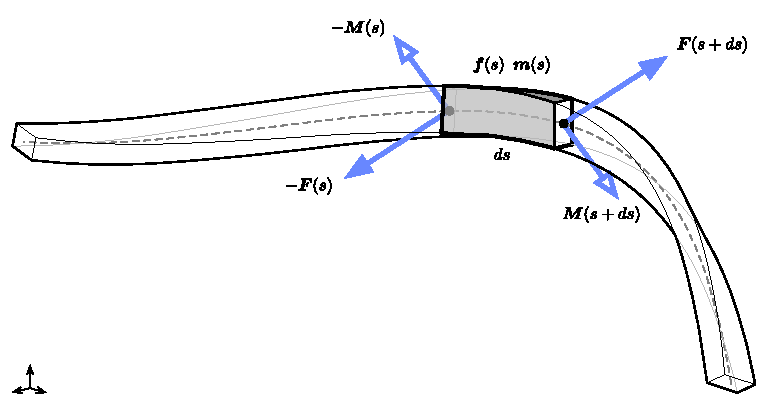
\includegraphics[]{kirchhoff_law.pdf}
	\caption{Internal forces ($\vect{F}$) and moments ($\vect{M}$) acting on an infinitesimal beam slice of length $ds$. The beam is also subject to distributed external forces ($\vect{f}$) and moments ($\vect{m}$).} By convention, internal forces and moments are forces and moments applied by the right part to the left part of the beam.
	\label{fig:5_0}
\end{figure}

\subsubsection{Reference (or stress-free) configuration}

We consider a \emph{stress-free} configuration of the rod that is called the \emph{reference} configuration.\footnote{See \cite[p.~20]{Audoly2010} for precisions when such a configuration may not exist.} The rod is fully described by its centerline ${\gamma}$ and its material frame $\{{\vect{d}_1}, {\vect{d}_2}, {\vect{d}_3}\}$.\footnote{We use the notation employed by Antman in his \emph{special Cosserat theory of rods} : \blockcquote[p.~270]{Antman2005}{The motion of a special Cosserat rod is defined by three vector-valued functions : $ [s_1, s_2] \times \mathbb{R} \ni  (s,t) \mapsto \vect{r}(s,t), \; \vect{d}_1 (s,t), \; \vect{d}_2 (s,t) \in \mathbb{E}^3$}. However, somme specific assumptions will be made over the directors in the context of Kirchhoff's theory.} The set of material points lying in a plane perpendicular to ${\gamma}$ defines a \emph{cross-section} ($\mathcal{S}$) and is thus a planar surface. 

We require that ${\gamma}$ is at least a regular space curve. We denote ${s}$ its arc length parameter, ${L}$ its length and $\rconf{\vect{x}}$ the position vector from some fixed origin :
\begin{equation}
	\fonctionL{{\gamma}}{[0,{L}]}{\mathbb{R}^3}{{s}}{\rconf{\vect{x}}({s})}
\end{equation}
As a regular curve, ${\gamma}$ is $\mathcal{C}^1$ and its tangent vector is continuously defined over [0,L] :
\begin{equation}
	{\vect{t}} = \frac{d \rconf{\vect{x}}}{d {s}}
\end{equation}
We also require that each cross-section centroid belong to the centerline. We choose ${\vect{d}_1}({s})$ and ${\vect{d}_2}({s})$ to be  unit vectors aligned with the principal axes of the cross-section $\mathcal{S}(s)$ so they are perpendicular to each other and lie in the plane of $\mathcal{S}({s})$ :
\begin{equation}
	\fonctionL{({\vect{d}_1},{\vect{d}_2})}{[0,{L}]}{\mathbb{R}^3 \times \mathbb{R}^3}{{s}}{({\vect{d}_1}({s}), {\vect{d}_2}({s}))} 
\end{equation}
For a sufficiently slender rod, the position of material point $\rconf{\vect{p}}$ in section $\mathcal{S}(s)$ can be expressed through its material coordinates $(X_1, X_2)$ as : \footnote{The lateral dimension of the rod must be smaller than the radius of curvature. Otherwise, this description would lead to self intersecting cross-sections.}
%\begin{equation}
%	\rconf{\vect{p}}({X_1}, {X_2}, {s}) = 
%	\rconf{\vect{x}}({s}) + {X_1} {\vect{d}_1}({s}) + {X_2} {\vect{d}_2}({s})
%\end{equation}
\begin{subequations}
	\begin{alignat}{2}
		&\rconf{\vect{p}}(X_1, X_2, s) &&= \rconf{\vect{x}}({s}) + \rconf{\vect{r}}(X_1, X_2, s)
		\\
		 &\rconf{\vect{r}}(X_1, X_2, s) &&=  X_1 \vect{d}_1 (s) + X_2 \vect{d}_2 (s)
	\end{alignat}
\end{subequations}
Consequently, for each $s$ in the reference configuration, $({X_1}, {X_2})$ is a cartesian coordinate system for the plane $\mathcal{S}(s)$. In this system the local coordinates of the section's centroid are $(0,0)$. The cross-section is assumed to be bounded and the boundary curve is defined by the equation : $f_s(X_1,X_2) = 0$.

Finally, we define the third component of the material frame as the unit vector so that $\{{\vect{d}_1}, {\vect{d}_2}, {\vect{d}_3}\}$ forms a direct orthonormal basis : 
\begin{equation}
	{\vect{d}_3} = {\vect{d}_1} \times {\vect{d}_2} = {\vect{t}}
\end{equation}
Since the material frame is orthonormal, it's evolution along the \emph{undeformed} centerline is described thanks to the \emph{reference strain vector} $\rconf{\vect{\omega}}$ defined as :
\begin{equation}
	\frac{d}{d s}\left(\vect{d}_i\right) = \rconf{\vect{\omega}}  \times \vect{d}_i
\end{equation}
In the reference configuration, because the centerline is parametrized by arc length, the strain vector components expressed in the material frame take the form :
\begin{subequations}
	\begin{alignat}{3}
		&\rconf{\omega}_1 &&= \rconf{\kappa}_1 &&= \rconf{\vect{\kappa b}} \cdot \vect{d}_1
		\\
		&\rconf{\omega}_2 &&= \rconf{\kappa}_2 &&= \rconf{\vect{\kappa b}} \cdot \vect{d}_2
		\\
		&\rconf{\omega}_3 &&= \rconf{\tau} &&= \vect{d}'_1  \cdot \vect{d}_2
	\end{alignat}
\end{subequations}
where $\rconf{\vect{\kappa b}}$ is the curvature binormal vector of $\gamma$ :
\begin{equation}
 	\rconf{\vect{\kappa b}} =  \vect{t} \times  \frac{\partial \vect{t}}{\partial s} = \vect{t} \times \vect{t}'
\end{equation}
$\rconf{\omega}_1$ and $\rconf{\omega}_2$ are called the \emph{material} or \emph{rod} reference curvatures. $\rconf{\omega}_3$ is called the \emph{material} or \emph{rod} reference twist. Note the important distinction with the geometric notions of curvature ($\kappa$) and twist ($\tau_f$) for space curves as defined in \cref{sec:spacecurve}.
\subsubsection{Actual (or deformed) configuration}

We now examine the motion of the rod and we call \emph{actual} or \emph{deformed} configuration its configuration at time $t$. In this configuration the rod undergoes internal stresses under body loads, external loads and constrains. 

The deformed configuration of the rod at time $t$ is now described by its centerline $\gamma_t = \gamma(t)$, its material frame $\{{\vect{d}_1}, {\vect{d}_2}, {\vect{d}_3}\}(t)$ and a local displacement field $\vect{u}_t = \vect{u}(t)$. A material point $\rconf{\vect{p}}$ in the \emph{reference} configuration is transported to position $\vect{p}_t = \vect{p}(t)$ in the \emph{actual} configuration so that :
\begin{subequations}
	\begin{alignat}{2}
		&\vect{p}(X_1, X_2, s, t) &&= \vect{x}(s,t) + \vect{r}(X_1, X_2, s, t)
		\\
		&\vect{r}(X_1, X_2, s, t) &&=  X_1 \vect{d}_1 (s,t) + X_2 \vect{d}_2 (s,t) + \vect{u}(X_1, X_2, s, t)
		\\
		&\vect{u}(X_1, X_2, s, t) &&=  \sum_{k=1}^3 u_k(X_1,X_2, s, t) \vect{d}_k (s, t)
	\end{alignat}
\end{subequations}
Although the cross-section $\mathcal{S}(s)$ is a planar surface in the \emph{reference} configuration, it deforms to a non-planar surface in the \emph{actual} configuration since $\vect{u} \neq \vect{0}$.\footnote{$\mathcal{S}(s)$ refers to the same set of material points in any configurations.} The components $(u_1, u_2, u_3)^T$ of the local displacement field expressed in the material frame basis are required to be small in Kirchhoff's theory of rods.\footnote{Note that this hypothesis is the one made by Kirchhoff and does not correspond to the well-known \emph{Euler-Bernoulli} or \emph{Navier-Bernoulli} assumption where the sections remain planar, undeformed and normal to the centerline during the rod deformation. In particular, torsion is responsible for the warping of cross-sections -- that is sections don't remain planar -- and leads to a distinct value of the twist modulus. This is clearly stipulated in \cite{Dill1992, Audoly2010} but is often treated with confusion in the literature.} In practice, as explained by \cite{Dill1992} this means that the considered motions must satisfy :
\begin{equation}
	\frac{u_i}{h} = O(\alpha)
	\quad , \quad
	\frac{\partial u_i}{\partial X_1} = O(\alpha)
	\quad , \quad
	\frac{\partial u_i}{\partial X_2} = O(\alpha)
	\quad , \quad
	\frac{\partial u_i}{\partial s} = O(\alpha^2)
\end{equation}
In this theory, the material frame in the reference configuration deforms in a rigid-body manner so that it remains orthonormal and aligned to the principal axes of the cross-section -- within an error $O(\alpha^2)$.\footnote{\blockcquote[p.~344]{Coleman1993}{[...] upon deformation, the principal axes of $\mathcal{S}(s)$ do remain normal to each other and to the rod axis, at least to within the approximations of the present theory, i.e., to within an error $O(\alpha^2).$}.} Remark that this is different than assuming that cross-sections deform in a rigid-body manner, which is known as the \emph{Euler-Bernoulli} hypothesis and is equivalent to the special case $\vect{u} = \vect{0}$.

The centerline of the rod is deformed into the space curve $\gamma_t$ with position vector $\vect{x}$ : 
\begin{equation}
	\fonctionL{\gamma_t}{[0,{L}]}{\mathbb{R}^3}{s}{\vect{x}(s,t)}
\end{equation}
The curve is still parametrized by $s$, the arc length parameter of the \emph{reference} configuration, as the constitutive laws will be expressed relatively to this configuration. But note that $s$ is no more the arc length parameter of the \emph{deformed} centerline as the rod may have suffer axial extension.\footnote{In Kirchhoff's theory, rods are not supposed to be strictly inextensible but extension has to remain small. Thus, the internal axial force is given by a constitutive law and not considered as a geometric constrained. However, some authors have remarked that it might be convenient and reasonable to solve the equations of motion considering the geometric contraint $\epsilon = 0$. See \cite[p.~98]{Audoly2010} for a detailed discussion of the subject.} Kirchhoff's theory assumes that the material frame remains adapted to the centerline during deformation, or equivalently that transverse shears are neglected.\footnote{This is also known as the \textquote{unsherable} assumption. Indeed, if $\frac{\partial \vect{x}}{\partial s} = \nu_k \vect{d}_k = (1 + \epsilon)\vect{d}_3 \Leftrightarrow \nu_1 = \nu_2 = 0$.} The extension of the centerline is characterized by $\epsilon$ defined such that :
 \begin{equation}
	\frac{\partial \vect{x}}{\partial s} = \nu_3 \vect{d}_3 =  (1 + \epsilon) \vect{d}_3
\end{equation}
However, one can parametrized the deformed centerline by its own arc length parameter, denoted $s_t$. We call $L_t$ the length of the deformed centerline and $g_t$ the $\mathcal{C}^1$ diffeomorphism that maps $s$ onto $s_t$ ($s_t = g_t(s) \Leftrightarrow s = g_t^{-1}(s_t)$). Thus, the centerline is also described as :
\begin{equation}
	\fonctionL{\gamma_t}{[0,{L_t}]}{\mathbb{R}^3}{s_t}{\vect{x}(s_t)}
\end{equation}
Because $s_t$ is the arc length parameter of $\gamma_t$ the following relations hold :
\begin{subequations}
	\begin{alignat}{2}
		&\frac{\partial \vect{x}}{\partial s_t} &&= \vect{t} = \vect{d}_3
		\\[0.5em]
		&\frac{\partial s_t}{\partial s} &&= \nu_3 = 1+ \epsilon
	\end{alignat}
\end{subequations}
Since the material frame is orthonormal, it's evolution along the \emph{deformed} centerline is described thanks to the \emph{actual strain vector} ${\vect{\omega}}$ defined as :
\begin{equation}
	\frac{\partial}{\partial s}\left(\vect{d}_i\right) = {\vect{\omega}}  \times \vect{d}_i
\end{equation}
Note that the strain vector is defined relatively to the arc length $s$ of the \emph{reference} configuration and not the arc length $s_t$ of the \emph{actual} configuration. Thus the strain vector components expressed in the material frame basis are given by :
\begin{subequations}
	\begin{alignat}{3}
		&{\omega}_1 &&= (1+\epsilon) {\kappa_1} &&= (1+\epsilon) \vect{\kappa b} \cdot \vect{d}_1
		\\
		&{\omega}_2 &&= (1+\epsilon) {\kappa_2} &&= (1+\epsilon) \vect{\kappa b} \cdot \vect{d}_2
		\\
		&{\omega}_3 &&= (1+\epsilon) {\tau} &&= (1+\epsilon) \frac{\partial \vect{d}_1}{\partial s_t}  \cdot \vect{d}_2
	\end{alignat}
\end{subequations}
where $\vect{\kappa b}$ is the curvature binormal vector of $\gamma_t$ given by :
\begin{equation}
 	\vect{\kappa b} =  \vect{t} \times  \frac{\partial \vect{t}}{\partial s_t} = (1+\epsilon) \vect{t} \times \vect{t}'
\end{equation}
${\omega}_1$ and ${\omega}_2$ are called the \emph{material} or \emph{rod} curvatures. ${\omega}_3$ is called the \emph{material} or \emph{rod} twist. Again, note the important distinction with the geometric notions of curvature ($\kappa$) and twist ($\tau_f$) for space curves as defined in \cref{sec:spacecurve}. In particular, the material strains ($\omega_1$, $\omega_2$, $\omega_3$) depend on the extension of the rod. These are the strains employed in the classical constitutive laws that lead to the determination of the internal axial force ($N = ES \epsilon$), internal bending moments ($M_1 = EI_1(\omega_1-\rconf{\omega}_1)$, $M_2 = EI_2(\omega_2-\rconf{\omega}_2)$) and internal twisting moment ($Q = GJ((\omega_3-\rconf{\omega}_3)$). 

In the case of an inextensible rod ($\epsilon = 0$) there is no need to make the distinction between $s_t$ and $s$. The same parameter is the arc length parameter for all configurations at all time.

\subsection{Balance of momentum}

Let $\vect{\mathcal{P}}$ be the first \emph{Piola-Kirchhoff} stress tensor. $\vect{\mathcal{P}}$ expresses how contact forces are acting in a \emph{deformed} body, referring to its (known) \emph{reference} configuration. Let $\vect{dS} =  \vect{n}dS$ be an elementary oriented surface of the rod in the \emph{reference} configuration of  centroid $\vect{p}(X_1,X_2,s,t) \in \mathcal{S}(s)$.\footnote{$dS$ is the area and $\vect{n}$ is the unit normal of the elementary oriented surface $\vect{dS}$.} The contact forces exerted on $\vect{dS}$ are given by :
\begin{subequations}
	\begin{alignat}{2}
		&\vect{dF}(X_1,X_2,s,t) &&=  \vect{\sigma_n}(X_1,X_2,s,t) \,dS 
		\\
		&\vect{\sigma_n}(X_1,X_2,s,t) &&= \vect{\mathcal{P}}(X_1,X_2,s,t) \cdot \vect{n} \label{eq:piola}
	\end{alignat}
\end{subequations}
We have introduce the \emph{Piola stress vector} ($\vect{\sigma_n}$) which expresses the contact forces exerted on the body per unit area of the \emph{reference} configuration.\footnote{For a detailed introduction to the Piola-Kirchhoff stress tensor, refer to \cite[p.~52]{Audoly2010}.}

The generic laws for the balance of linear and angular momentums are obtained by summation over the reference configuration, where $\vect{b}$ are the body forces per unit volume of the \emph{reference} configuration :
\begin{subequations}
	\begin{alignat}{2}
		&\iiint_{\mathcal{V}} \rho \ddot{\vect{p}} \;dV 
		&&= \iint_{\partial\mathcal{V}} \vect{\sigma_n} \;dS 
		+ \iiint_{\mathcal{V}} \rho \vect{b} \;dV
		\label{eq:linearbalance}
		\\[0.5em]
		&\iiint_{\mathcal{V}} \rho (\vect{p} \times \ddot{\vect{p}}) \;dV  
		&&=  \iint_{\partial\mathcal{V}} \vect{p} \times \vect{\sigma_n} \;dS 
		+ \iiint_{\mathcal{V}} \rho (\vect{p} \times \vect{b}) \;dV
		\label{eq:angularbalance}
	\end{alignat}
\end{subequations}
Here, and subsequently, $\mathcal{V}$ denotes the volume of a slice of the rod in the \emph{reference} configuration, encompassed between two cross-sections ($\mathcal{S}_1 = \mathcal{S}(s_1)$, $\mathcal{S}_2 = \mathcal{S}(s_2)$, $s_1 < s_2$). We also denote $\mathcal{L}_{12}$ the lateral surface of the rod in the \emph{reference} configuration so that the exterior surface of the volume is : $\partial \mathcal{V} = \mathcal{S}_1 \bigcup \mathcal{L}_{12} \bigcup \mathcal{S}_2$.

The cross-section $\mathcal{S}(s)$ splits the rod in two parts. Hereafter, the upstream part of the rod over $[s,L]$ we will called the \textquote{right part}. Reciprocally, the downstream part of the rod over $[0,s]$ will be called the \textquote{left part}.

\subsubsection{Internal forces and moments}
At the cross-section $\mathcal{S}(s)$, the contact forces applied by the right part onto the left part of the rod yield the following resultant force $\vect{F}$ and resultant moment $\vect{M}$ about the point $\vect{x}(s,t)$ :
\begin{subequations}
	\begin{alignat}{2}
		&\vect{F}(s, t) &&= \iint_{\mathcal{S}(s)} \vect{\sigma_n}(X_1, X_2, s, t) \;dX_1 dX_2 \label{eq:F}
		\\[0.5em]
		&\vect{M}(s, t) &&= \iint_{\mathcal{S}(s)} \vect{r}(X_1,X_2,s,t) \times \vect{\sigma_n}(X_1, X_2, s, t) \;dX_1 dX_2 \label{eq:M}
	\end{alignat}
\end{subequations}
$\vect{F}$ and $\vect{M}$ are commonly known as the \emph{internal forces} and the \emph{internal moments} of the rod.

\subsubsection{External forces and moments}
We assume that the resultant distributed force and moment of the contact forces on $\mathcal{L}_{12}$ and the body forces on $\mathcal{V}$ reduced to the following forms :
\begin{subequations}
	\begin{alignat}{2}
		&\iint_{\mathcal{L}} \vect{\sigma_n} \;dS 
		+ \iiint_{\mathcal{V}} \rho \vect{b} \;dV
		= \int_s \rconf{\vect{f}} + (1+\epsilon) \vect{f}_t \;ds
		\label{eq:f}
		\\[0.5em]
		&\iint_{\mathcal{L}} \vect{p} \times \vect{\sigma_n} \;dS 
		+ \iiint_{\mathcal{V}} \rho (\vect{p} \times \vect{b}) \;dV
		= \int_s \rconf{\vect{m}} + (1+\epsilon) \vect{m}_t + \vect{x} \times \big(\rconf{\vect{f}} + (1+\epsilon) \vect{f}_t \big) \;ds
		\label{eq:m}
	\end{alignat}
\end{subequations}
where $\rconf{\vect{f}}$  (resp. $\vect{f_t}$) is the distributed resultant force per unit length of the reference (resp. deformed) configuration ; and $\rconf{\vect{m}}$  (resp. $\vect{m}_t$) is the distributed resultant moment per unit length of the reference (resp. deformed) configuration. For instance, these distributed forces and moments include external and body loads such as weight, snow, wind, ... \footnote{At this stage, although this is uncommon in the literature, it has been found convenient to mark the distinction between loads referring to the reference configuration and loads referring to the actual configuration. Indeed, various distributed loads depend on the actual length of an element such as pressure and wind loads. On the other hand, some loads are independent of the extension of the rod, such as its weight.}

Note that Kirchhoff's theory require that the stress components on the sides of the rod are small \cite[p.~11]{Dill1992} -- that is $\vect{\sigma_n}\cdot \vect{n} = O(\alpha^2)$ over $\mathcal{L}$. Thus, the first two terms in the above expression will be neglected :
\begin{subequations}
	\begin{alignat}{2}
		&\iint_{\mathcal{L}} \vect{\sigma_n} \;dS \simeq 0
		\\[0.5em]
		&\iint_{\mathcal{L}} \vect{p} \times \vect{\sigma_n} \;dS \simeq 0
	\end{alignat}
\end{subequations}
Although the continuous model does not account formally for punctual loads,\footnote{This is possible but would require more math. However, local effects of such loads would not be properly modeled in the theory of Kirchhoff (Saint-Venant's Principle).} they will be introduced seamlessly in the discrete model as the dynamical equations for the motion of the rod will translate into rigid body equations for the discrete segments composing the rod.

\subsubsection{Inertial forces}
The inertial forces for a volume of the rod encompassed between cross-sections $\mathcal{S}_1$ and $\mathcal{S}_2$ are obtained by summation as : 
\begin{subequations}
	\begin{alignat}{2}
		&\iiint_{\mathcal{V}} {\rho} \ddot{\vect{p}} \;dV = \iiint_{\mathcal{V}_t} {\rho_t} \ddot{\vect{p}} \;dV_t \label{eq:inertial_a}
		\\[0.5em]
		&\iiint_{\mathcal{V}} \rho (\vect{p} \times \ddot{\vect{p}}) \;dV= \iiint_{\mathcal{V}_t} {\rho_t} (\vect{p} \times  \ddot{\vect{p}}) \;dV_t \label{eq:inertial_b}
	\end{alignat}
\end{subequations}
Here, ${\rho}$ (resp. ${\rho_t}$) is the mass density of the rod in the reference (resp. deformed) configuration. Expressions are given in both coordinate systems.\footnote{In \cite{Dill1992} the change in volume and the conservation of mass is expressed through the determinants of the metric tensors of the reference and deformed configurations. Recall that this determinant is the square of the volume of the elementary cell defined by $\frac{\partial \vect{p}}{\partial s}$, $\frac{\partial \vect{p}}{\partial X_1}$, $\frac{\partial \vect{p}}{\partial X_2}$ in the reference configuration, which is convected to the elementary cell defined by $\frac{\partial \vect{p}_t}{\partial s}$, $\frac{\partial \vect{p}_t}{\partial X_1}$, $\frac{\partial \vect{p}_t}{\partial X_2}$ in the reference configuration.}

In the context of Kirchhoff's approximation, the local deformations of the cross-sections can be neglected in the computation of the inertial forces \cite[p.~16]{Dill1992}. This yields :
\begin{subequations}
	\begin{alignat}{2}
		&\vect{p} &&\simeq \vect{x} + X_1\vect{d}_1 + X_2\vect{d}_2
		\\
		&\dot{\vect{p}} &&= \dot{\vect{x}} + \vect{\mathrm{w}} \times (X_1\vect{d}_1 + X_2\vect{d}_2)
		\\
		&\ddot{\vect{p}} &&= \ddot{\vect{x}} + \dot{\vect{\mathrm{w}}} \times (X_1\vect{d}_1 + X_2\vect{d}_2) + \vect{\mathrm{w}} \times ( \vect{\mathrm{w}} \times (X_1\vect{d}_1 + X_2\vect{d}_2))
	\end{alignat}
\end{subequations}
Since $X_1$ and $X_2$ are the coordinates with respect to the centroid ($\vect{x}$) and the principal axes of the cross-section ($\vect{d}_1$, $\vect{d}_2$), the cross-section area ($S$) and principal moments of inertia ($I_1$, $I_2$) are given by : \footnote{This is exact in the reference configuration but only approximately true in the deformed configuration as the theory consider only small deformations of cross-sections.}\textsuperscript{,}\footnote{\cref{eq:centroid_a} is nothing but the definition of the centroid position. \cref{eq:diag} holds because the tensor of inertia of the cross-section is diagonal in the basis $\{\vect{d}_1, \vect{d}_2, \vect{d}_3\}$ and thus $I_{12} = I_{21} = 0$.}
\begin{subequations}
\label{eq:sectionprop}
	\begin{alignat}{2}
		&0  		&&= \iint_{\mathcal{S}(s)} \left(X_1 X_2\right) \;dX_1 dX_2 \label{eq:diag}
		\\
		&S 		&&= \iint_{\mathcal{S}(s)} dX_1 dX_2
		\\
		&I_1 		&&= \iint_{\mathcal{S}(s)} {X_2}^2 \;dX_1 dX_2
		\\
		&I_2 		&&= \iint_{\mathcal{S}(s)} {X_1}^2 \;dX_1 dX_2
	\end{alignat}
\end{subequations}
More over, for a given cross-section the definition of the centroid yields :
\begin{subequations}
\label{eq:centroid}
	\begin{alignat}{2}
		&\vect{0}  &&= \iint_{\mathcal{S}(s)} \left(X_1\vect{d}_1 + X_2\vect{d}_2\right) \;dX_1 dX_2 \label{eq:centroid_a}
		\\
		&0 		&&= \iint_{\mathcal{S}(s)} {X_1} \;dX_1 dX_2 \label{eq:centroid_b}
		\\
		&0 		&&= \iint_{\mathcal{S}(s)} {X_2} \;dX_1 dX_2 \label{eq:centroid_c}
	\end{alignat}
\end{subequations}
For a thin slice of the rod ($\delta\mathcal{V}$) between cross-sections $\mathcal{S}(s)$ and $\mathcal{S}(s+ds)$, \cref{eq:inertial_a,eq:inertial_b} yield respectively : \footnote{Indeed, since $\iint_{\mathcal{S}(s)} \vect{r} \;dX_1 dX_2 = \vect{0}$ from \cref{eq:centroid_a} we have $\iint_{\mathcal{S}(s)} \ddot{\vect{r}} \;dX_1 dX_2 =  \iint_{\mathcal{S}(s)} \dot{\vect{\mathrm{w}}} \times \vect{r} + \vect{\mathrm{w}} \times ( \vect{\mathrm{w}} \times \vect{r}) \; dX_1 dX_2 = \vect{0}$ and $\iint_{\mathcal{S}(s)} \vect{r} \times \ddot{\vect{x}} \; dX_1 dX_2 = \vect{0}$ as $\vect{w}$ and $\vect{x}$ are independent of $X_1$ and $X_2$.}
\begin{subequations}
	\begin{alignat}{2}
		&\iiint_{\delta\mathcal{V}} {\rho} \ddot{\vect{p}} \;dV= ({\rho}S \ddot{\vect{x}})ds
		\\[0.5em]
		&\iiint_{\delta\mathcal{V}} \rho (\vect{p} \times \ddot{\vect{p}}) \;dV= \left({\rho}S \ddot{\vect{x}} + {\rho} \iint_{\mathcal{S}(s)} \vect{r} \times \ddot{\vect{r}} \; dX_1 dX_2 \right)ds
	\end{alignat}
\end{subequations}
Finally, remark that :
\begin{equation}
	\vect{r} \times \ddot{\vect{r}}
	= (X_1)^2 \vect{d}_1 \times \ddot{\vect{d}_1} 
	+ (X_2)^2 \vect{d}_2 \times \ddot{\vect{d}_2} 
	+ X_1 X_2 (\vect{d}_1 \times \ddot{\vect{d}_2} 
	+ \vect{d}_2 \times \ddot{\vect{d}_1})
\end{equation}
Thus, reminding \cref{eq:sectionprop,eq:centroid}, one can conclude that the inertial forces reduce to :
\begin{subequations}
	\begin{alignat}{2}
		&\iiint_{\delta\mathcal{V}} {\rho} \ddot{\vect{x}} \;dV= ({\rho}S \ddot{\vect{x}})ds \label{eq:linearinertia}
		\\[0.5em]
		&\iiint_{\delta\mathcal{V}} \rho (\vect{p} \times \ddot{\vect{p}}) \;dV = ({\rho}S \ddot{\vect{x}} + \rho I_1 \vect{d}_1 \times \ddot{\vect{d}_1} + \rho I_2 \vect{d}_2 \times \ddot{\vect{d}_2}) ds \label{eq:angularinertia}
	\end{alignat}
\end{subequations}

\subsubsection{Balance of linear momentum}
For a thin slice of the rod ($\delta\mathcal{V}$) between cross-sections $\mathcal{S}(s)$ and $\mathcal{S}(s+ds)$, using \cref{eq:F,eq:f}, the balance of linear momentum referring to the \emph{reference} configuration expressed in \cref{eq:linearbalance} yields : 
\begin{equation}
	\begin{aligned}
		\iiint_{\delta\mathcal{V}} \rho \ddot{\vect{p}} \;dV 
		&= \iint_{\partial\mathcal{V}} \vect{\sigma_n} \;dS 
		+ \iiint_{\delta\mathcal{V}} \rho \vect{b} \;dV
		\\[0.5em]
		&= \iint_{\mathcal{S}(s)} \vect{\sigma_n} \;dS 
		+ \iint_{\mathcal{S}(s+ds)} \vect{\sigma_n} \;dS
		+ \left( \iint_{\delta\mathcal{L}} \vect{\sigma_n} \;dS
		+ \iiint_{\delta\mathcal{V}} \rho \vect{b} \;dV \right)
		\\[0.5em]
		&= -\vect{F}(s) + \vect{F}(s+ds) + \big(\rconf{\vect{f}}(s) + (1+\epsilon) \vect{f}_t(s) \big) ds
		\\[0.5em]
		&= \left( \frac{\partial \vect{F}}{\partial s} + \rconf{\vect{f}} + (1+\epsilon) \vect{f}_t \right)(s) ds
	\end{aligned}
\end{equation}
Thus, using \cref{eq:linearinertia}, the equation for the balance of linear momentum reduce to either equations :
\begin{subequations}
	\begin{alignat}{1}
	\frac{\partial \vect{F}}{\partial s} + \rconf{\vect{f}} + (1+\epsilon)\vect{f}_t &= \rho S \ddot{\vect{x}}
	\label{eq:linearmotion}
	\\[0.5em]
	(1+\epsilon)\frac{\partial \vect{F}}{\partial s_t} + \rconf{\vect{f}} + (1+\epsilon)\vect{f}_t &= \rho S \ddot{\vect{x}}
	\end{alignat}
\end{subequations}

\subsubsection{Balance of angular momentum}
Similarly, for a thin slice of the rod ($\delta\mathcal{V}$) between cross-sections $\mathcal{S}(s)$ and $\mathcal{S}(s+ds)$, using \cref{eq:F,eq:M} yields : 
\begin{equation}
	\begin{aligned}
		\iint_{\mathcal{S}(s) \bigcup \mathcal{S}(s+ds)} \vect{p} \times \vect{\sigma_n} \;dS
		&= \iint_{\mathcal{S}(s) \bigcup \mathcal{S}(s+ds)} (\vect{x} + \vect{r}) \times \vect{\sigma_n} \;dS
		\\[0.5em]
		&= -(\vect{x}\times\vect{F})(s) + (\vect{x}\times\vect{F})(s+ds) - \vect{M}(s) + \vect{M}(s+ds)
		\\[0.5em]
		&=  \frac{\partial}{\partial s} \big( \vect{M} + \vect{x}\times\vect{F} \big)(s) ds
	\end{aligned}
\end{equation}
Using \cref{eq:m}, the balance of linear momentum referring to the \emph{reference} configuration expressed in \cref{eq:angularbalance} yields : 
\begin{equation}
	\label{eq:angularbalance2}
	\begin{aligned}
		\iiint_{\delta\mathcal{V}} \rho (\vect{p} \times \ddot{\vect{p}}) \;dV  
		&=  \iint_{\partial\delta\mathcal{V}} \vect{p} \times \vect{\sigma_n} \;dS 
		+ \iiint_{\delta\mathcal{V}} \rho (\vect{p} \times \vect{b}) \;dV
		\\[0.5em]
		&= \frac{\partial}{\partial s} \big( \vect{M} + \vect{x}\times\vect{F} \big)(s) ds 
		+ \rconf{\vect{m}} + (1+\epsilon)\vect{m}_t + \vect{x} \times \big(\rconf{\vect{f}} + (1+\epsilon)\vect{f}_t \big) \;ds 
	\end{aligned}
\end{equation}
Finally, combining \cref{eq:angularbalance2} with \cref{eq:linearmotion,eq:angularinertia}, the equation for the balance of angular momentum reduce to either equations : \footnote{Note the simplification of the term $\rho S \ddot{\vect{x}}$. Alternatively, the balance equations could be written for the slice as for a rigid body. In the barycentric frame of the slice : $\frac{d}{dt}(dI_G) = \vect{M}(s+ds)-\vect{M}(s) + \vect{m}(s)ds + (\tfrac{1}{2}ds\vect{x}')\times \vect{F}(s+ds) + (-\tfrac{1}{2}ds\vect{x}')\times -\vect{F}(s) = \left(\frac{\partial \vect{M}}{\partial s}(s)+\vect{m}(s) + \vect{x}'\times \vect{F}(s)\right)ds$ with $dI_G \simeq \rho ds (I_1 \vect{d}_1 + I_2 \vect{d}_2 + (I_1+I_2) \vect{d}_3)$.}
\begin{subequations}
	\begin{alignat}{1}
	\frac{\partial \vect{M}}{\partial s} 
	+ \frac{\partial \vect{x}}{\partial s} \times \vect{F}
	+ \rconf{\vect{m}} + (1+\epsilon)\vect{m}_t 
	&= \rho I_1 \vect{d}_1 \times \ddot{\vect{d}_1} + \rho I_2 \vect{d}_2 \times \ddot{\vect{d}_2}
	\\[0.5em]
	(1+\epsilon)\frac{\partial \vect{M}}{\partial s_t} 
	+ (1+\epsilon)\frac{\partial \vect{x}}{\partial s_t} \times \vect{F}
	+ \rconf{\vect{m}} + (1+\epsilon) \vect{m}_t 
	&= \rho I_1 \vect{d}_1 \times \ddot{\vect{d}_1} + \rho I_2 \vect{d}_2 \times \ddot{\vect{d}_2}
	\end{alignat}
\end{subequations}

\subsection{Equations of motion}
With some scaling arguments \cite{Dill1992} shows that terms in $w_1$ and $w_2$ should be negligible in the inertial forces of the rod given in \cref{eq:angularinertia}, which yields to : \footnote{\blockcquote[p. 17]{Dill1992}{It follows that $\omega_1$ and $\omega_2$ can be neglected in the kinetic energy [\ldots]. However, $\omega_3$, which provides the angular momentum about the axis of the rod, must be retained, This assumption of Kirchhoff is consistent with the technical theory of beams where rotary inertia is known to provide corrections to the natural frequencies of vibration of $O(\alpha^2)$ if the length measure is the half-wave length}. This assumption is made in numerous publications but often with ambiguous or no justifications, as of instance : \blockcquote[]{Casati2013}{neglecting inertial momentum due to the vanishing cross-section lead to the following dynamic equations for a Kirchhoff rod}.}
\begin{subequations}
	\begin{alignat}{1}
	\rho I_1 (\dot{w}_1 + w_2 w_3) &\simeq 0
	\\
	\rho I_2 (\dot{w}_2 - w_1 w_3) &\simeq 0
	\\
	\rho (I_1 + I_2)\dot{w}_3 +\rho(I_1 - I_1)w_1 w_2 &\simeq \rho (I_1 + I_2)\dot{w}_3
	\end{alignat}
\end{subequations}
For our application -- a beam model for quasi-static analysis of gridshell structures -- this approximation is clearly sufficient as what matters is the quasi-static response of the structural system and there is no need for a too accurate modeling of the transient phase. More over, the quasi-static response will be determined through a fictitious dynamic process appropriately damped to speed up the convergence to the steady state, and so there is no reason that the transient phase has any real physical meaning. This means that its is enough to keep only the twisting dynamic of the rod around its centerline.

Thus, the final dynamical equations for the motion of the rod to be retained are :
\begin{subequations}
	\begin{alignat}{1}
	\frac{\partial \vect{F}}{\partial s} + \rconf{\vect{f}} + (1+\epsilon) \vect{f}_t 
	&= \rho S \ddot{\vect{x}}
	\\[0.5em]
	\frac{\partial \vect{M}}{\partial s} 
	+ \frac{\partial \vect{x}}{\partial s} \times \vect{F}
	+ \rconf{\vect{m}} + (1+\epsilon) \vect{m}_t 
	&\simeq \rho (I_1 + I_2)\dot{w}_3 \vect{d}_3
	\end{alignat}
\end{subequations}

\subsection{Hookean elasticity}

From now on we consider that the rod material is isotropic and linear elastic.\footnote{This is true at first order for small strains anyway.} This is the framework of the so called \emph{Hookean Elasticity}. This assumption allows the determination of the local displacement field ($\vect{u}$), the strain tensor ($\tens{E}$), the stress tensor ($\tens{S}$) and the constitutive equations that link the axial force ($\vect{F}_1$), the bending moments ($\vect{M}_1$, $\vect{M}_2$) and the twisting moment ($\vect{M}_3$) to the strains ($\epsilon$, $\vect{\omega}$, $\rconf{\vect{\omega}}$).

Such a material is characterized by a linear relation between the strain and stress tensors that takes the form : \footnote{Using Einstein notation this expression yields : $\sigma_{ij} = \lambda \epsilon_{kk} \delta_{ij} + 2\mu\epsilon_{ij}$.}
\begin{equation}
	\tens{S} = 2\mu\tens{E} + \lambda \Tr{\tens{E}} \tens{I}
\end{equation}
where $\lambda$ and $\mu$ are known as the elastic coefficients of Lamé. This coefficients are related to the elastic ($E$) and shear ($G$) modulus and to the Poisson ratio ($\nu$) :
\begin{subequations}
	\begin{alignat}{1}
	\mu &= \frac{E}{2(1+\nu)} = G
	\\[0.5em]
	\lambda &= \frac{2\mu\nu}{1-2\nu}
	\end{alignat}
\end{subequations}
A worthwhile presentation of the theory of elasticity in the specific context of rods can be found in \cite{Audoly2010}.

\subsection{Deformation of cross-sections}
\begin{figure}[t]
	\centering
	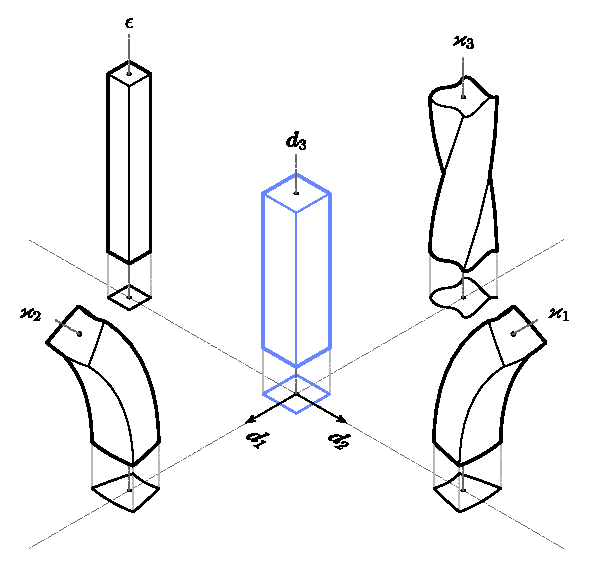
\includegraphics[]{kirchhoff_cross_section_deformation.pdf}
	\caption{Typical deformations of cross-sections in Kirchhoff's theory.}
	\label{fig:section_defo}
\end{figure}


In this paragraph, we simply recall the canonical form of the local displacement field ($\vect{u}$) for the cross-section $\mathcal{S}(s)$ in the context of Kirchhoff's approximation : \footnote{Remark that the local displacement field results from the superposition of the three displacement fields obtained for pure and uniform extension, flexion and twist. For a detailed analysis of pure and uniform flexion and twist of rods; refer to \cite[ch.~3]{Audoly2010}.}
\begin{subequations}
	\begin{alignat}{1}
	u_1 &=
	-\nu \epsilon X_1 
	- \nu(\omega_1 - \rconf{\omega}_1) X_1 X_2
	+ \tfrac{1}{2}\nu(\omega_2 - \rconf{\omega}_2)({X_1}^2 - {X_2}^2)
	\\[0.5em]
	u_2 &= 
	-\nu \epsilon X_2 
	+ \nu(\omega_2 - \rconf{\omega}_2) X_1 X_2
	+ \tfrac{1}{2}\nu(\omega_1 - \rconf{\omega}_1)({X_1}^2 - {X_2}^2)
	\\[0.5em]
	u_3 &= (\omega_3 - \rconf{\omega}_3)\varphi_s(X_1,X_2)
	\end{alignat}
\end{subequations}
where $\varphi_s$ is the warping function (in torsion) of $\mathcal{S}(s)$, determined by the differential equation and the boundary condition over the contour of the cross-section : \footnote{$\vect{n} = ({\partial f_s}/{\partial {X_1}}, {\partial f_s}/{\partial {X_1}})^T$ is the unit normal vector to the boundary curve of $\mathcal{S}(s)$ defined implicitly by the equation $f_s(X_1,X_2)=0$.}
\begin{subequations}
	\begin{alignat}{2}
	0 &= \frac{\partial^2 \varphi_s}{\partial {X_1}^2} + \frac{\partial^2 \varphi_s}{\partial {X_2}^2}
	&& \forall (X_1,X_2)\in\mathcal{S}(s)
	\\[0.5em]
	0 &= \frac{\partial f_s}{\partial {X_1}}\left(\frac{\partial \varphi_s}{\partial {X_1}} - X_2 \right) 
	+ \frac{\partial f_s}{\partial {X_2}}\left(\frac{\partial \varphi_s}{\partial {X_2}} + X_1 \right)
	&& \forall (X_1,X_2)\in\mathcal{S}(s)\; / \; f_s(X_1,X_2) = 0
	\end{alignat}
\end{subequations}
These equations have known analytical solutions for classical shapes such as circles, ellipses, squares or rectangles. For other shapes, when it is not easy to find analytical solutions, the membrane analogy introduced by Prandtl \cite{Prandtl1903} is employed.\footnote{Recent advances \cite{Koohestani2014} in the formfinding of soap films with the force density method might be of practical use to evaluate the warping function.}

\subsection{Strains}
In this paragraph, we simply recall the canonical form of the strain tensor ($\tens{E}$) for the cross-section $\mathcal{S}(s)$ in the context of Kirchhoff's approximation : 
\begin{subequations}
	\begin{alignat}{1}
	\epsilon_{33} &= \epsilon + (\omega_1 - \rconf{\omega}_1) X_2 - (\omega_2 - \rconf{\omega}_2) X_1 \label{eq:strain_a}
	\\
	\epsilon_{11} &=  \epsilon_{22} = -\nu \epsilon_{33}	\label{eq:strain_b}
	\\
	\epsilon_{12} &= 0 \label{eq:strain_c}
	\\
	\epsilon_{31} &= \tfrac{1}{2}(\omega_3 - \rconf{\omega}_3)\left(\frac{\partial \varphi_s}{\partial {X_1}} - X_2 \right) \label{eq:strain_d}
	\\
	\epsilon_{32} &= \tfrac{1}{2}(\omega_3 - \rconf{\omega}_3)\left(\frac{\partial \varphi_s}{\partial {X_2}} + X_1 \right) \label{eq:strain_e}
	\end{alignat}
\end{subequations}

\subsection{Stresses}
In this paragraph, we simply recall the canonical form of the strain tensor ($\tens{E}$) for the cross-section $\mathcal{S}(s)$ in the context of Kirchhoff's approximation : 
\begin{subequations}
	\begin{alignat}{1}
	\sigma_{33} &= E \epsilon_{33} \label{eq:stress_a}
	\\
	\sigma_{11} &=  \sigma_{22} = \sigma_{12} = 0 \label{eq:stress_b}
	\\
	\sigma_{31} &= 2G \epsilon_{31}	\label{eq:stress_c}
	\\
	\sigma_{32} &= 2G \epsilon_{32}	\label{eq:stress_d}
	\end{alignat}
\end{subequations}
Thus, the Piola stress vector defined in \cref{eq:piola} becomes :
\begin{equation}
	\vect{\sigma_n} = \sigma_{31}\vect{d}_1 + \sigma_{32}\vect{d}_2 + \sigma_{33}\vect{d}_3 \label{eq:piola2}
\end{equation}

\subsection{Constitutive equations for internal forces and moments}
In Kirchhoff's theory, constitutive equations for internal forces and moments should not be considered as assumptions. Indeed, as shown hereafter, they are somehow consequences of the assumptions made on the motion -- that is the rod remains close to a motion where cross-sections remain planar, undistorted and perpendicular to the centerline -- and on the material -- the Hookean elasticity -- of the rod.

From \cref{eq:F,eq:piola2,eq:stress_a,eq:strain_a} we deduce the constitutive equation for the axial component of the internal forces : \footnote{Also recall from \cref{eq:centroid} that $\iint_{\mathcal{S}(s)} {X_1} \;dX_1 dX_2 = 0$ and $\iint_{\mathcal{S}(s)} {X_2} \;dX_1 dX_2 = 0$.}
\begin{equation}
%	\label{eq:constitutive_F3}
	\begin{aligned}
		F_3 &= \iint_{\mathcal{S}(s)} \vect{\sigma_n}(X_1, X_2, s, t) \cdot \vect{d}_3 \;dX_1 dX_2 
		\\[0.5em]
		&= ES\epsilon 
		- (\omega_2 - \rconf{\omega}_2) \iint_{\mathcal{S}(s)} {X_1} \;dX_1 dX_2
		+ (\omega_1 - \rconf{\omega}_1) \iint_{\mathcal{S}(s)} {X_2} \;dX_1 dX_2
		\\[0.5em]
		&= ES\epsilon
	\end{aligned}
\end{equation}
From \cref{eq:M,eq:piola2,eq:stress_c,eq:stress_d,eq:strain_e,eq:strain_d} we deduce the constitutive equation for the axial component of the internal moments : 
\begin{equation}
% 	\label{eq:constitutive_M3}
	\begin{aligned}
		M_3 &= \iint_{\mathcal{S}(s)} (\vect{r} \times \vect{\sigma_n}(X_1, X_2, s, t)) \cdot \vect{d}_3 \;dX_1 dX_2
		\\[0.5em]
		&= \iint_{\mathcal{S}(s)} -X_2\sigma_{31} + X_1\sigma_{32}  \;dX_1 dX_2 
		\\[0.5em]
		&= G (\omega_3 - \rconf{\omega}_3) 
		\iint_{\mathcal{S}(s)} X_1 \left( \frac{\partial \varphi_s}{\partial {X_2}} + X_1 \right ) - X_2 \left( \frac{\partial \varphi_s}{\partial {X_1}}  - X_2 \right )
		 \;dX_1 dX_2 
	\end{aligned}
\end{equation}
From \cref{eq:M,eq:piola2,eq:stress_a,eq:strain_a} we deduce the constitutive equation for the first component of the internal moments : 
\begin{equation}
% 	\label{eq:constitutive_M3}
	\begin{aligned}
		M_1 &= \iint_{\mathcal{S}(s)} (\vect{r} \times \vect{\sigma_n}(X_1, X_2, s, t)) \cdot \vect{d}_1 \;dX_1 dX_2
		\\[0.5em]
		&= \iint_{\mathcal{S}(s)} X_2\sigma_{33} \;dX_1 dX_2 
		\\[0.5em]
		&= E (\omega_1 - \rconf{\omega}_1) \iint_{\mathcal{S}(s)} {X_2}^2  \;dX_1 dX_2 
	\end{aligned}
\end{equation}
From \cref{eq:M,eq:piola2,eq:stress_a,eq:strain_a} we deduce the constitutive equation for the second component of the internal moments : 
\begin{equation}
% 	\label{eq:constitutive_M3}
	\begin{aligned}
		M_2 &= \iint_{\mathcal{S}(s)} (\vect{r} \times \vect{\sigma_n}(X_1, X_2, s, t)) \cdot \vect{d}_2 \;dX_1 dX_2
		\\[0.5em]
		&= \iint_{\mathcal{S}(s)} - X_1\sigma_{33} \;dX_1 dX_2 
		\\[0.5em]
		&= E (\omega_2 - \rconf{\omega}_2) \iint_{\mathcal{S}(s)} {X_1}^2  \;dX_1 dX_2 
	\end{aligned}
\end{equation}

\clearpage
\subsection{Summary of the theory}
Let's summarize the assumptions and results of Kirchhoff's theory of rods on which our discret beam model will be based on.

In the reference configuration the rod is described by its reference strains :
\begin{equation}
	\vect{d}'_i= \rconf{\vect{\omega}}  \times \vect{d}_i
\end{equation}
In the actual configuration the rod is described by its strains and spin vector :
\begin{subequations}
	\begin{alignat}{1}
	\vect{x}' &= (1+\epsilon)\vect{t}
	\\
	\vect{d}'_i&= {\vect{\omega}}  \times \vect{d}_i
	\\
	\ddot{\vect{d}_i}&= {\vect{w}}  \times \vect{d}_i
	\end{alignat}
\end{subequations}
The rod is subjected to internal forces and moments :
\begin{subequations}
	\begin{alignat}{1}
	\vect{F} &= F_1\vect{d}_1 + F_2\vect{d}_2 + F_3\vect{d}_3
	\\
	\vect{M} &= M_1\vect{d}_1 + M_2\vect{d}_2 + M_3\vect{d}_3
	\end{alignat}
\end{subequations}
The rod is subjected to external and body loads described as distributed forces and moments acting on the centerline -- either given per unit length of the reference configuration ($\rconf{\vect{f}}$, $\rconf{\vect{m}}$) or per unit length of the actual configuration ($\vect{f}_t$, $\vect{m}_t$) -- and given in the condensed form :
\begin{subequations}
	\begin{alignat}{1}
	\vect{f} &= \rconf{\vect{f}} + (1+\epsilon)\vect{f}_t = f_1\vect{d}_1 + f_2\vect{d}_2 + f_3\vect{d}_3
	\\
	\vect{m} &= \rconf{\vect{m}} + (1+\epsilon)\vect{m}_t = m_1\vect{d}_1 + m_2\vect{d}_2 + m_3\vect{d}_3
	\end{alignat}
\end{subequations}
The internal axial force, the internal bending moments and the internal twisting moment are computed with the following constitutive equations :
\begin{subequations}
	\begin{alignat}{1}
	F_3 &= ES\epsilon
	\\
	M_1 &= EI_1(\omega_1 - \rconf{\omega}_1)
	\\
	M_2 &= EI_2(\omega_2 - \rconf{\omega}_2)
	\\
	M_3 &= GJ(\omega_3 - \rconf{\omega}_3)
	\end{alignat}
\end{subequations}
where $S$, $I_1$, $I_2$, $J$ are respectively the area, the second moments of inertia and the torsional stiffness of the cross-section :
\begin{subequations}
	\begin{alignat}{2}
	&S 	&&= \iint_{\mathcal{S}(s)} dX_1 dX_2
	\\
	&I_1	&&= \iint_{\mathcal{S}(s)} {X_2}^2 \;dX_1 dX_2
	\\
	&I_2	&&= \iint_{\mathcal{S}(s)} {X_1}^2 \;dX_1 dX_2
	\\
	&J 	&&= \iint_{\mathcal{S}(s)} X_1 \left( \frac{\partial \varphi_s}{\partial {X_2}} + X_1 \right ) - X_2 \left( \frac{\partial \varphi_s}{\partial {X_1}}  - X_2 \right )
			\;dX_1 dX_2 
	\end{alignat}
\end{subequations}
and $\varphi_s$ is the warping fonction of the cross-section that satisfies the differential system : 
\begin{subequations}
	\begin{alignat}{2}
	0 &= \frac{\partial^2 \varphi_s}{\partial {X_1}^2} + \frac{\partial^2 \varphi_s}{\partial {X_2}^2}
	&\;,\;& \forall (X_1,X_2)\in\mathcal{S}(s)
	\\[0.5em]
	0 &= \frac{\partial f_s}{\partial {X_1}}\left(\frac{\partial \varphi_s}{\partial {X_1}} - X_2 \right) 
	+ \frac{\partial f_s}{\partial {X_2}}\left(\frac{\partial \varphi_s}{\partial {X_2}} + X_1 \right)
	&\;,\;&\forall (X_1,X_2)\; / \; f_s(X_1,X_2) = 0
	\end{alignat}
\end{subequations}
The dynamical equations for the motion of the rod are :
\begin{subequations}
	\begin{alignat}{1}
	\frac{\partial \vect{F}}{\partial s} + \vect{f} 
	&= \rho S \ddot{\vect{x}}
	\\[0.5em]
	\frac{\partial \vect{M}}{\partial s} 
	+ \frac{\partial \vect{x}}{\partial s} \times \vect{F}
	+ \vect{m} 
	&= \rho I_1 \vect{d}_1 \times \ddot{\vect{d}_1} + \rho I_2 \vect{d}_2 \times \ddot{\vect{d}_2}
	\end{alignat}
\end{subequations}
Neglecting the rotational dynamics around $\vect{d}_1$ and $\vect{d}_2$ the components of the above equations are written :
\begin{subequations}
	 \label{eq:motion}
	\begin{alignat}{1}
	F'_1 + \omega_2 F_3 - \omega_3 F_2 + f_1 &= \rho S \ddot{x}_1  \label{eq:motion_1}
	\\
	F'_2 + \omega_3 F_1 - \omega_1 F_3 + f_2 &= \rho S \ddot{x}_2 \label{eq:motion_2}
	\\
	F'_3 + \omega_1 F_2 - \omega_2 F_1 + f_3 &= \rho S \ddot{x}_3 \label{eq:motion_3}
	\\
	M'_1 + \omega_2 M_3 - \omega_3 M_2 - (1+\epsilon)F_2  + m_1 & \simeq 0 \label{eq:motion_4}
	\\
	M'_2 + \omega_3 M_1 - \omega_1 M_3 + (1+\epsilon)F_1 + m_2 & \simeq 0 \label{eq:motion_5}
	\\
	M'_3 + \omega_1 M_2 - \omega_2 M_1 + m_3 & \simeq \rho (I_1 + I_2)\dot{w}_3 \label{eq:motion_6}
	\end{alignat}
\end{subequations}
The local displacements of the cross-sections are given by :
\begin{subequations}
	\begin{alignat}{1}
	u_1 &=
	-\nu \epsilon X_1 
	- \nu(\omega_1 - \rconf{\omega}_1) X_1 X_2
	+ \tfrac{1}{2}\nu(\omega_2 - \rconf{\omega}_2)({X_1}^2 - {X_2}^2)
	\\[0.5em]
	u_2 &= 
	-\nu \epsilon X_2 
	+ \nu(\omega_2 - \rconf{\omega}_2) X_1 X_2
	+ \tfrac{1}{2}\nu(\omega_1 - \rconf{\omega}_1)({X_1}^2 - {X_2}^2)
	\\[0.5em]
	u_3 &= (\omega_3 - \rconf{\omega}_3)\varphi_s(X_1,X_2)
	\end{alignat}
\end{subequations}
The non-zero components of the strain tensor are given by :
\begin{subequations}
	\begin{alignat}{1}
	\epsilon_{33} &= \epsilon + (\omega_1 - \rconf{\omega}_1) X_2 - (\omega_2 - \rconf{\omega}_2) X_1
	\\
	\epsilon_{31} &= \tfrac{1}{2}(\omega_3 - \rconf{\omega}_3)\left(\frac{\partial \varphi_s}{\partial {X_1}} - X_2 \right)
	\\
	\epsilon_{32} &= \tfrac{1}{2}(\omega_3 - \rconf{\omega}_3)\left(\frac{\partial \varphi_s}{\partial {X_2}} + X_1 \right)
	\\
	\epsilon_{11} &=  \epsilon_{22} = -\nu \epsilon_{33}
	\end{alignat}
\end{subequations}
The non-zero components of the stress tensor are given by :
\begin{subequations}
	\begin{alignat}{1}
	\sigma_{33} &= E \epsilon_{33} 
	\\
	\sigma_{31} &= 2G \epsilon_{31}
	\\
	\sigma_{32} &= 2G \epsilon_{32}
	\end{alignat}
\end{subequations}

\subsection{Comments}

\begin{itemize}
\item 
The internal shear forces are reacting parameters and are given by the balance equations. Transverse shear deformations and stresses are not given by the present theory.
\item
There is a noticeable symmetry in the equations between the roles played by $F_1$, $F_2$ and $M_1$, $M_2$ and by the roles played by $F_2$ and $M_3$.
\item
Warping is supposed to happen freely.
\end{itemize}



\clearpage
\makebox[\textwidth]{} % necessaire pour le saut de page et le flush des floats
\newpage
\section{Geometric interpretation of Kirchhoff's equations}

The previous equations for the motion of the rod (see \cref{eq:motion_1,eq:motion_2,eq:motion_3,eq:motion_4,eq:motion_5,eq:motion_6}) have been established expressing the fundamental principles of balance of linear and angular momentums. An alternative approach, leading to the same results, consists in differentiating the elastic energy of a given configuration of the rod -- assumed to be stationary -- with respect to the degrees of freedom of the mechanical system (principle of virtual work).\footnote{This is the approach employed in the theory presented in \cref{sec:capter 4} and is also the one developed in \cite{Audoly2010}, for strictly inextensible rods.} 
\\
However, the approach through equilibrium seems easier to understood as it is (almost) just a matter of balance between forces and moments on infinitesimal slices of the rods (see \cref{fig:slice}). This is of obvious pedagogical interest as it allows to understand how the geometry of the rod influence the splitting of the elastic energy between extension, flexion and torsion of the rod.
\\
To emphasis this, we provide the proper drawings (see \cref{fig:kb,fig:d1,fig:d2}) and computations for the contribution of internal forces and moments to the balance of linear and angular momentums. This is what we call the \textquote{geometric interpretation} of Kirchhoff's equations.

\begin{figure}[h]
	\centering
	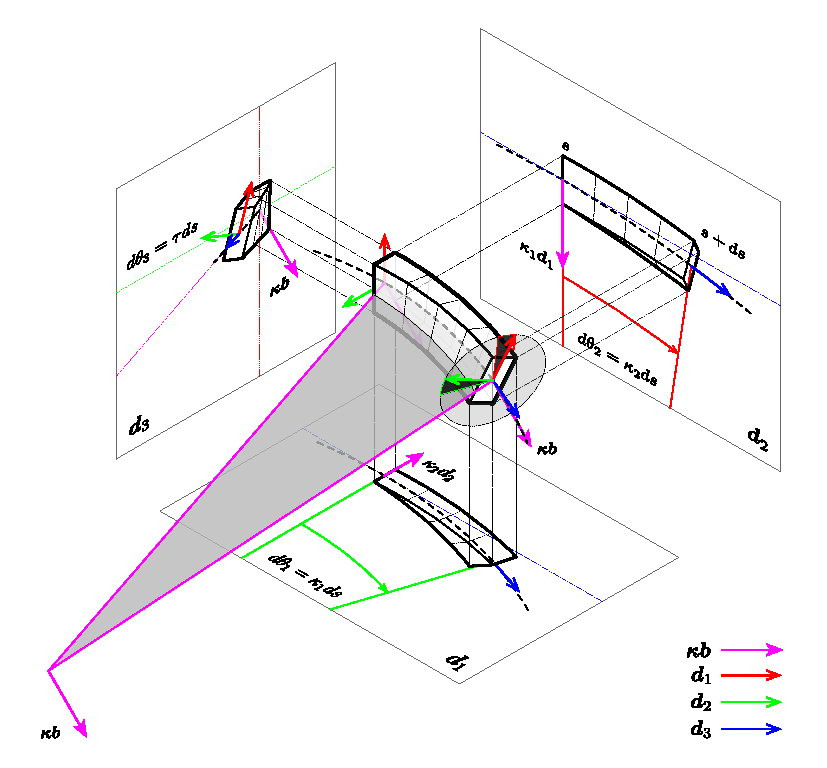
\includegraphics[]{kirchhoff_geometry.pdf}
	\caption{Flexion and torsion of an elementary slice of a Kirchhoff rod of length $ds$. Projections of the deformations are given in the material planes defined by $\vect{d}_1$, $\vect{d}_2$, $\vect{d}_3$.}
	\label{fig:slice}
\end{figure} 

\begin{figure}[p]
  \begin{leftfullpage}
    \captionsetup[subfloat]{captionskip=10pt}
     	\centering
     	\subfloat[][Infinitesimal deformation.]{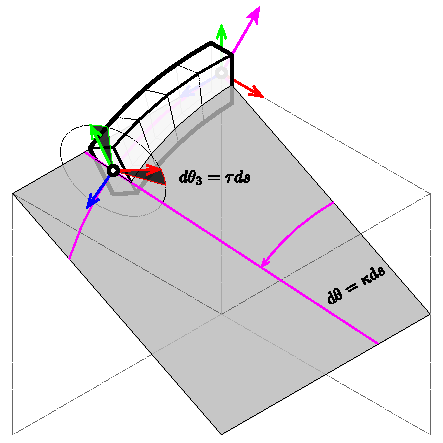
\includegraphics{kirchhoff_geometry_kb.pdf}\label{fig:kb_a}} \\
	\vspace{30pt}
	\subfloat[][Contributions of the internal forces.]{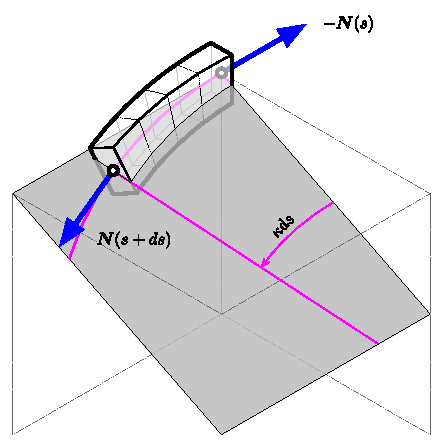
\includegraphics{kirchhoff_balance_T_kb.pdf}\label{fig:kb_b}}
	\subfloat[][Contributions of the internal moments.]{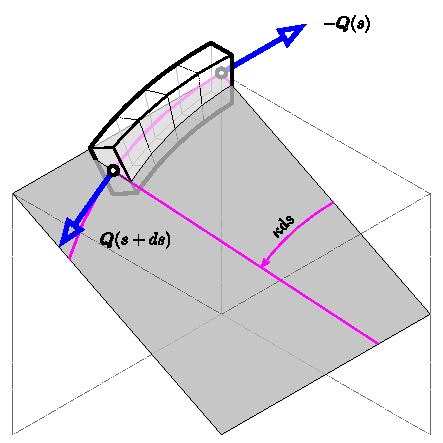
\includegraphics{kirchhoff_balance_M_kb.pdf}\label{fig:kb_c}}
	\vspace{30pt}
	\caption{Influence of the curvature ($\kappa$) in the deflection of internal forces and moments along the centerline.}     
	\label{fig:kb}
 \end{leftfullpage}
\end{figure}
\begin{figure}[p]
	\begin{fullpage}
	\subsubsection{Contributions to the balance of forces}
	\vspace{10pt}
	$\vect{N}(s+ds)$ is deflected from $\vect{d}_3(s)$ by the rotation of angle $\kappa ds$ around $\vect{\kappa b}$ (\cref{fig:kb_b}). Thus, its contribution to the balance of forces onto $\vect{d}_3(s)$ is : 
	\begin{equation*}
		N(s+ds) \cos(\kappa ds) - N(s) = N'(s) ds + o(ds)
	\end{equation*}	
	\vspace{10pt}
	
	\subsubsection{Contributions to the balance of moments}
	\vspace{10pt}
	$\vect{Q}(s+ds)$ is deflected from $\vect{d}_3(s)$ by the rotation of angle $\kappa ds$ around $\vect{\kappa b}$ (\cref{fig:kb_c}). Thus, its contribution to the balance of moments onto $\vect{d}_3(s)$ is : 
	\begin{equation*}
		Q(s+ds) \cos(\kappa ds) - Q(s) = Q'(s) ds + o(ds)
	\end{equation*}	
	  \end{fullpage}
\end{figure}

% ============
 
\begin{figure}[p]
  \begin{leftfullpage}
    \captionsetup[subfloat]{captionskip=10pt}
     	\centering
     	\subfloat[][Infinitesimal deformation.]{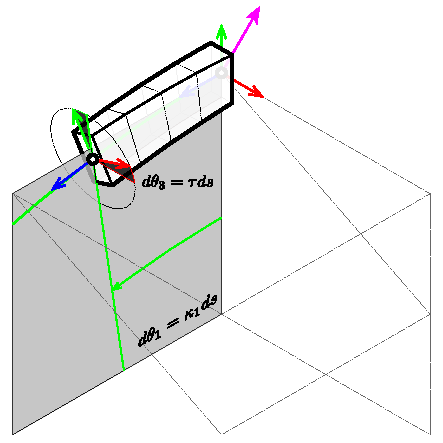
\includegraphics{kirchhoff_geometry_d1.pdf}\label{fig:d1_a}} \\
	\vspace{30pt}
	\subfloat[][Contributions of the internal forces.]{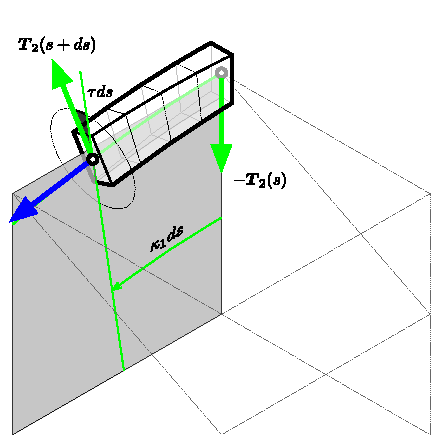
\includegraphics{kirchhoff_balance_T_d1.pdf}\label{fig:d1_b}}
	\subfloat[][Contributions of the internal moments.]{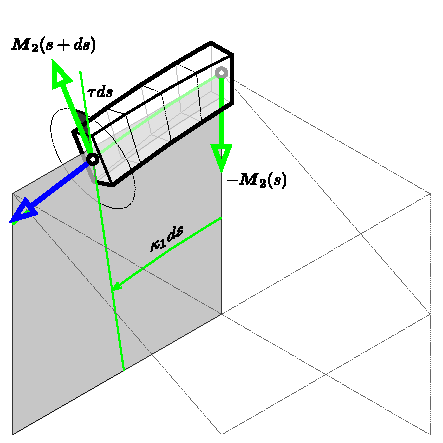
\includegraphics{kirchhoff_balance_M_d1.pdf}\label{fig:d1_c}}
	\vspace{30pt}
	\caption{Influence of the first material curvature ($\kappa_1$) in the deflection of internal forces and moments along the centerline.}     
	\label{fig:d1}
 \end{leftfullpage}
\end{figure}
\begin{figure}[p]
	\begin{fullpage}
	\subsubsection{Contributions to the balance of forces}
	\vspace{10pt}
	
	$\vect{T}_2(s+ds)$ is deflected from $\vect{d}_2(s)$ by the combined rotations of angle $\tau ds$ around $\vect{d}_3$ and $\kappa_2 ds$ around $\vect{d}_2$ (\cref{fig:d1_b}). Thus, its contribution to the balance of forces onto $\vect{d}_1(s)$ is : 
	\begin{equation*}
		-T_2(s+ds) \sin(\tau ds) \cos(\kappa_2 ds) = -\tau T_2(s) ds + o(ds)
	\end{equation*}	
	
	$\vect{T}_2(s+ds)$ is deflected from $\vect{d}_2(s)$ by the combined rotations of angle $\tau ds$ around $\vect{d}_3$ and $\kappa_1 ds$ around $\vect{d}_1$ (\cref{fig:d1_b}). Thus, its contribution to the balance of forces onto $\vect{d}_2(s)$ is : 
	\begin{equation*}
		-T_2(s) + T_2(s+ds) \cos(\tau ds) \cos(\kappa_1 ds) = T'_2 (s) ds + o(ds)
	\end{equation*}	
	
	$\vect{T}_2(s+ds)$ is deflected from $\vect{d}_2(s)$ by the combined rotations of angle $\tau ds$ around $\vect{d}_3$ and $\kappa_1 ds$ around $\vect{d}_1$ (\cref{fig:d1_b}). Thus, its contribution to the balance of forces onto $\vect{d}_3(s)$ is : 
	\begin{equation*}
		T_2(s+ds) \cos(\tau ds) \sin(\kappa_1 ds) = \kappa_1 T_2(s) ds + o(ds)
	\end{equation*}
		
	$\vect{N}(s+ds)$ is deflected from $\vect{d}_3(s)$ by the combined rotations of angle $\kappa_2 ds$ around $\vect{d}_2$ and $\kappa_1 ds$ around $\vect{d}_1$ (\cref{fig:d1_b}). Thus, its contribution to the balance of forces onto $\vect{d}_2(s)$ is : 
	\begin{equation*}
		-N(s+ds) \cos(\kappa_2 ds) \sin(\kappa_1 ds) = -\kappa_1 N(s) ds + o(ds)
	\end{equation*}	
	\vspace{10pt}

	\subsubsection{Contributions to the balance of moments}
	\vspace{10pt}
	
	$\vect{T}_2(s+ds)$ is deflected from the plane normal to $\vect{d}_1(s)$ by a rotation of angle $\tau ds$ around $\vect{d}_3$ (\cref{fig:d1_b}). It produces a moment around $\vect{d}_1$ with the lever arm $b =  \cos(\kappa_2 ds) ds$. Thus, its contribution to the balance of moments onto $\vect{d}_1(s)$ is : 
	\begin{equation*}
		-T_2(s+ds) \cos(\tau ds) (\cos(\kappa_2 ds) ds) = -T_2(s) ds + o(ds)
	\end{equation*}
	
	$\vect{M}_2(s+ds)$ is deflected from $\vect{d}_2(s)$ by the combined rotations of angle $\tau ds$ around $\vect{d}_3$ and $\kappa_2 ds$ around $\vect{d}_2$ (\cref{fig:d1_c}). Thus, its contribution to the balance of moments onto $\vect{d}_1(s)$ is : 
	\begin{equation*}
		-M_2(s+ds) \sin(\tau ds) \cos(\kappa_2 ds) = -\tau M_2 (s) ds + o(ds)
	\end{equation*}	
	
	$\vect{M}_2(s+ds)$ is deflected from $\vect{d}_2(s)$ by the combined rotations of angle $\tau ds$ around $\vect{d}_3$ and $\kappa_1 ds$ around $\vect{d}_1$ (\cref{fig:d1_c}). Thus, its contribution to the balance of moments onto $\vect{d}_2(s)$ is : 
	\begin{equation*}
		-M_2(s) + M_2(s+ds) \cos(\tau ds) \cos(\kappa_1 ds) = M'_2 (s) ds + o(ds)
	\end{equation*}
	
	$\vect{M}_2(s+ds)$ is deflected from $\vect{d}_2(s)$ by the combined rotations of angle $\tau ds$ around $\vect{d}_3$ and $\kappa_1 ds$ around $\vect{d}_1$ (\cref{fig:d1_c}). Thus, its contribution to the balance of moments onto $\vect{d}_3(s)$ is : 
	\begin{equation*}
		M_2(s+ds) \cos(\tau ds) \sin(\kappa_1 ds) = \kappa_1 M_2 (s) ds + o(ds)
	\end{equation*}	
	
	$\vect{Q}(s+ds)$ is deflected from $\vect{d}_3(s)$ by the combined rotations of angle $\kappa_2 ds$ around $\vect{d}_2$ and $\kappa_1 ds$ around $\vect{d}_1$ (\cref{fig:d1_c}). Thus, its contribution to the balance of moments onto $\vect{d}_2(s)$ is : 
	\begin{equation*}
		-Q(s+ds) \cos(\kappa_2 ds) \sin(\kappa_1 ds) = -\kappa_1 Q(s) ds + o(ds)
	\end{equation*}	
	  \end{fullpage}
\end{figure}

% ============
 
\begin{figure}[p]
  \begin{leftfullpage}
    \captionsetup[subfloat]{captionskip=10pt}
     	\centering
     	\subfloat[][Infinitesimal deformation.]{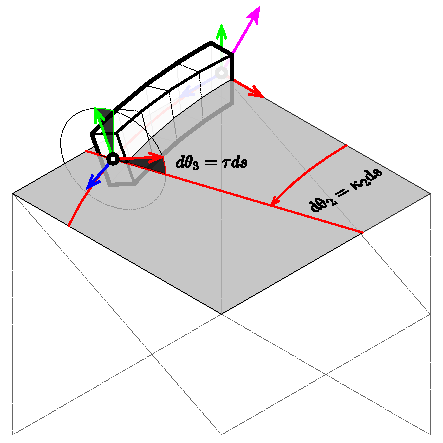
\includegraphics{kirchhoff_geometry_d2.pdf}\label{fig:d2_a}} \\
	\vspace{30pt}
	\subfloat[][Contributions of the internal forces.]{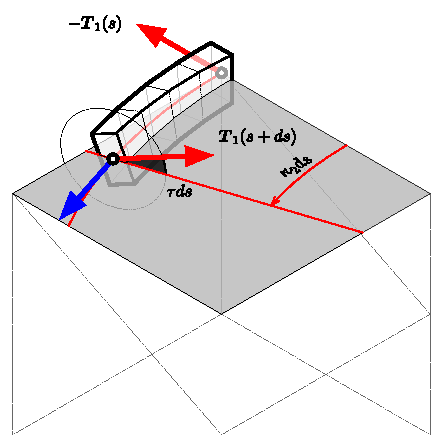
\includegraphics{kirchhoff_balance_T_d2.pdf}\label{fig:d2_b}}
	\subfloat[][Contributions of the internal moments.]{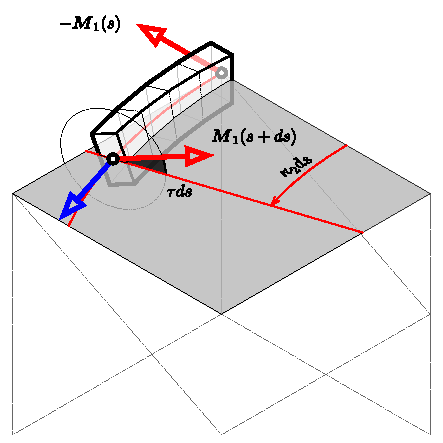
\includegraphics{kirchhoff_balance_M_d2.pdf}\label{fig:d2_c}}
	\vspace{30pt}
	\caption{Influence of the second material curvature ($\kappa_2$) in the deflection of internal forces and moments along the centerline.}     
	\label{fig:d2}
 \end{leftfullpage}
\end{figure}
\begin{figure}[p]
	\begin{fullpage}
	\subsubsection{Contributions to the balance of forces}
	\vspace{10pt}
	
	$\vect{T}_1(s+ds)$ is deflected from $\vect{d}_1(s)$ by the combined rotations of angle $\tau ds$ around $\vect{d}_3$ and $\kappa_2 ds$ around $\vect{d}_2$ (\cref{fig:d2_b}). Thus, its contribution to the balance of forces onto $\vect{d}_1(s)$ is : 
	\begin{equation*}
		-T_1(s) + T_1(s+ds) \cos(\tau ds) \cos(\kappa_2 ds) = T'_1 (s) ds + o(ds)
	\end{equation*}
	
	$\vect{T}_1(s+ds)$ is deflected from $\vect{d}_1(s)$ by the combined rotations of angle $\tau ds$ around $\vect{d}_3$ and $\kappa_1 ds$ around $\vect{d}_1$ (\cref{fig:d2_b}). Thus, its contribution to the balance of forces onto $\vect{d}_2(s)$ is : 
	\begin{equation*}
		T_1(s+ds) \sin(\tau ds) \cos(\kappa_1 ds) = \tau T_1 (s) ds + o(ds)
	\end{equation*}	
	
	$\vect{T}_1(s+ds)$ is deflected from $\vect{d}_1(s)$ by the combined rotations of angle $\tau ds$ around $\vect{d}_3$ and $\kappa_2 ds$ around $\vect{d}_2$ (\cref{fig:d2_b}). Thus, its contribution to the balance of forces onto $\vect{d}_3(s)$ is : 
	\begin{equation*}
		-T_1(s+ds) \cos(\tau ds) \sin(\kappa_2 ds) = - \kappa_2 T_1(s) ds + o(ds)
	\end{equation*}	
	
	$\vect{N}(s+ds)$ is deflected from $\vect{d}_3(s)$ by the combined rotations of angle $\kappa_1 ds$ around $\vect{d}_1$ and $\kappa_2 ds$ around $\vect{d}_2$ (\cref{fig:d2_b}). Thus, its contribution to the balance of forces onto $\vect{d}_1(s)$ is : 
	\begin{equation*}
		N(s+ds) \cos(\kappa_1 ds) \sin(\kappa_2 ds) = \kappa_2 N(s) ds + o(ds)
	\end{equation*}
	\vspace{10pt}

	\subsubsection{Contributions to the balance of moments}
	\vspace{10pt}
	
		$\vect{T}_1(s+ds)$ is deflected from the plane normal to $\vect{d}_2(s)$ by the angle $\tau ds$ around $\vect{d}_3$ along $ds$ (\cref{fig:d2_b}). It produces a moment around $\vect{d}_2$ with the lever arm $b =  \cos(\kappa_1 ds) ds$. Thus, its contribution to the balance of moments onto $\vect{d}_2(s)$ is : 
	\begin{equation*}
		T_1(s+ds) \cos(\tau ds) (\cos(\kappa_1 ds) ds) = T_1(s) ds + o(ds)
	\end{equation*}
	
	$\vect{M}_1(s+ds)$ is deflected from $\vect{d}_1(s)$ by the combined rotations of angle $\tau ds$ around $\vect{d}_3$ and $\kappa_2 ds$ around $\vect{d}_2$ (\cref{fig:d2_c}). Thus, its contribution to the balance of moments onto $\vect{d}_1(s)$ is : 
	\begin{equation*}
		-M_1(s) + M_1(s+ds) \cos(\tau ds) \cos(\kappa_2 ds) = M'_1 (s) ds + o(ds)
	\end{equation*}	
	
	$\vect{M}_1(s+ds)$ is deflected from $\vect{d}_1(s)$ by the combined rotations of angle $\tau ds$ around $\vect{d}_3$ and $\kappa_2 ds$ around $\vect{d}_2$ (\cref{fig:d2_c}). Thus, its contribution to the balance of moments onto $\vect{d}_2(s)$ is : 
	\begin{equation*}
		M_1(s+ds) \sin(\tau ds) \cos(\kappa_2 ds) = \tau M_1 (s) ds + o(ds)
	\end{equation*}	
	
	$\vect{M}_1(s+ds)$ is deflected from $\vect{d}_1(s)$ by the combined rotations of angle $\tau ds$ around $\vect{d}_3$ and $\kappa_2 ds$ around $\vect{d}_2$ (\cref{fig:d2_c}). Thus, its contribution to the balance of moments onto $\vect{d}_3(s)$ is : 
	\begin{equation*}
		-M_1(s+ds) \cos(\tau ds) \sin(\kappa_2 ds) = -\kappa_2 M_1 (s) ds + o(ds)
	\end{equation*}	
	
	$\vect{Q}(s+ds)$ is deflected from $\vect{d}_3(s)$ by the combined rotations of angle $\kappa_1 ds$ around $\vect{d}_1$ and $\kappa_2 ds$ around $\vect{d}_2$ (\cref{fig:d2_c}). Thus, its contribution to the balance of moments onto $\vect{d}_1(s)$ is : 
	\begin{equation*}
		Q(s+ds) \cos(\kappa_1 ds) \sin(\kappa_2 ds) = \kappa_2 Q(s) ds + o(ds)
	\end{equation*}	
	  \end{fullpage}
\end{figure}

\clearpage
\section{Numerical resolution}

\subsection{Main hypothesis}

On néglige les forces d'inertie liées à la rotation de l'élément  (devant quoi ?? traitement quasi-statique par rapport à la rotation). Cette hypothèse est faite explicitement chez Florence Bertail :



Cette hypothèse est faite mais passée sous silence chez Douthe, Adriaenssen, D'Amico lorsqu'ils déduisent l'effort tranchant du moment de flexion.

Principe :

- les équations constitutives permettent le calcul de $M_1$, $M_2$, $Q$ à partir de la géométrie $\{\vect{x},\theta\}$.

- La seconde loi de kirchhoff projetée sur les axes matériels 1 et 2 de la section me donnent accès aux efforts tranchants $T_1$ et $T_2$.

- La seconde loi de kirchhoff projetée sur les axes matériel 3 (tangente à la centerline) de la section me donnent l"hypothèse quasi-statique de Audoly.

%\begin{figure}[t]
%	\centering
%	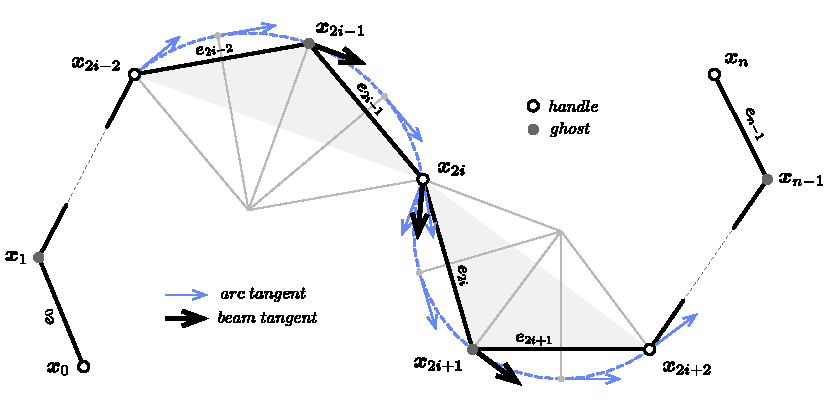
\includegraphics[]{discrete_model.pdf}
%	\caption{Biarc model for a discrete beam. The centerline is divided into curved segments (grey solid hatch). Each segment is defined as a 3-noded element with uniform material and section properties. It has two end vertices (white) called \emph{handle} as they are used to interact with the model, for instance to apply loads or restrains. It has one mid vertex (grey) called \emph{ghost} as it is used only to enrich the segment kinematics and is not accessible to the end user.}
%	\label{fig:discrete_model}
%\end{figure} 


\begin{figure}[p]
\begin{fullpage}
	\captionsetup[subfloat]{captionskip=20pt}
     	\centering
     	\subfloat[][Centerline of the discrete biarc model.]{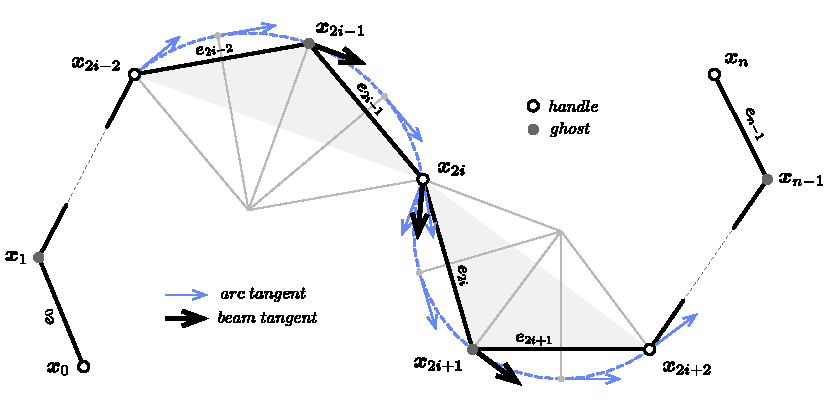
\includegraphics{discrete_model.pdf}\label{fig:discrete_model}} \\
	\vspace{30pt}
	\subfloat[][Number of segments, edges and vertices whether the centerline is closed or open.]{
		\begin{tabular}{l  l | c  c } 
		 &  & open & closed \\
		\hline
		segments & $n_s$ & $n_s$ & $n_s$ \\
		\hline
		edges & $n_e$ & $2 n_s$ & $2 n_s$ \\
		\hline
		vertices & $n$ & $2 n_s + 1$ & $2 n_s$ \\
		\hline
		ghosts & $n_g$ & $n_s$ & $n_s$ \\
		\hline
		handles & $n_h$ & $n_s+1$ & $n_s$ \\
	\end{tabular}\label{tab:count}}
	\vspace{20pt}
	\caption{Biarc model for a discrete beam. The centerline is divided into curved segments (grey solid hatch). Each segment is defined as a three-noded element with uniform material and section properties. It has two end vertices (white) called \emph{handle} as they are used to interact with the model, for instance to apply loads or restrains. It has one mid vertex (grey) called \emph{ghost} as it is used only to enrich the segment kinematics and is not accessible to the end user.}
\end{fullpage}
\end{figure}



\clearpage
\subsection{Discret beam model}
% =======================



Let's introduce the discrete biarc model to describe the configuration of a beam. It is composed of a discrete curve called \emph{centerline} and a discrete adapted frame called \emph{material frame} as its axes are chosen to be the principal axes of the beam cross-section (\cref{fig:discrete_model}). The centerline itself is organized in $n_s$ consecutive adjacent segments which are three-vertices and two-edges elements with uniform material and section properties.

Beams can either be closed or open. The corresponding number of vertices, edges and segments are reported in \cref{tab:count}.
%\begin{table}[h]
%	\centering
%	\begin{tabular}{l  l | c  c } 
%		 &  & open & closed \\
%		\hline
%		segments & $n_s$ & $n_s$ & $n_s$ \\
%		\hline
%		edges & $n_e$ & $2 n_s$ & $2 n_s$ \\
%		\hline
%		vertices & $n$ & $2 n_s + 1$ & $2 n_s$ \\
%		\hline
%		ghosts & $n_g$ & $n_s$ & $n_s$ \\
%		\hline
%		handles & $n_h$ & $n_s+1$ & $n_s$ \\
%	\end{tabular}
%\caption{Number of segments, edges and vertices whether the centerline is closed or open.}
%\label{tab:count}
%\end{table}

\subsubsection{Centerline}

The discrete centerline is a polygonal space curve (\cref{fig:discrete_model}) defined as an ordered sequence of $n+1$ pairwise disjoint \emph{vertices} : $\Gamma = (\vect{x}_0,  \vect{x}_1, \ldots, \vect{x}_n) \in \mathbb{R}^{3(n+1)}$. Consecutive pairs of vertices define $n$ straight segments $(\vect{e}_0,  \vect{e}_1, \ldots, \vect{e}_{n-1})$ called \emph{edges} and pointing from one vertex to the next one : $\vect{e}_i = \vect{x}_{i+1} - \vect{x}_{i}$ : 
\begin{equation}
%\setlength{\jot}{8pt}
	\left\{
	\begin{aligned}
		\vect{e}_i 	&= \vect{x}_{i+1} - \vect{x}_{i} \\
		l_i 		&= \norm{\vect{e}_i} \\
		\vect{u}_i 	&= \vect{e}_i / l_i\\
	\end{aligned}
	\right.
\end{equation}

The length of the ith edge is denoted $l_i $ and its normalized direction vector is denoted $\vect{u}_i$. The arc length of the ith vertex is denoted $s_i$ and is given by : 
\begin{equation}
	\left\{
	\begin{aligned}
		s_0 	&= 0 				& 	&i = 0		\\
		s_i 	&= \sum_{k=0}^{i-1} l_k	&	&i \in \llbracket 1, n-1 \rrbracket	\\
		s_n 	&=  L 				&	&i = n		\\
	\end{aligned}
	\right.
\end{equation}
Thus, the centerline is parametrized by arc length and $\Gamma(s_i) = \vect{x}_i$. Additionally, we define the vertex-based mean length at vertex $\vect{x}_i$ : 
\begin{equation}
%\setlength{\jot}{8pt}
	\left\{
	\begin{aligned}
		\rconf{l_0} 	& =  \tfrac{1}{2}l_0				&		&i = 0					\\
		\rconf{l_i}	& =  \tfrac{1}{2}(l_{i-1} + l_i)		&		&i \in \llbracket 1, n-1 \rrbracket	\\
		\rconf{l_n} 	& =  \tfrac{1}{2}l_{n-1} 			&		&i = n					\\
	\end{aligned}
	\right.
\end{equation}

\subsubsection{Segments}

The discrete centerline is divided into $n_s$ curved segments. Each segment is a three-noded element -- see \cref{fig:discrete_model} where the area covered by a segment is represented as a grey solid hatch. The ith segment is composed of three vertices ($\vect{x}_{2i}, \vect{x}_{2i+1},  \vect{x}_{2i+2}$) spanning two edges ($\vect{e}_{2i}, \vect{e}_{2i+1}$). The (i-1)th segment and the ith segment share the same vertex $\vect{x}_{2i}$ at arc length $s_{2i}$.

Each segment has two end vertices called \emph{handle} ($\vect{x}_{2i}, \vect{x}_{2i+2}$) and one mid vertex called \emph{ghost} ($\vect{x}_{2i+1}$) as this one is not accessible to the end user in order to interact with the model (link, restrain, loading, ...). Ghost vertices are used only for internal purpose to give a higher richness in the kinematic description of a segment than a two-noded segment would.

We define the \emph{chord length} of the ith segment as the distance between $\vect{x}_{2i}$ and $\vect{x}_{2i+2}$ : $L_i = \norm{\vect{e}_{2i} + \vect{e}_{2i+1}}$.

\subsubsection{Material and section properties}

In addition, the model assumes that a segment has uniform section ($S$, $I_1$, $I_2$, $J$)\footnote{$S$ is the cross-section area ; $I_1$, $I_2$ and $J$ are the cross-section principal moments of inertia.} and material ($E$, $G$)\footnote{$E$ is the elastic modulus and $G$ is the shear  modulus for the considered material} properties over its length : $s \in ]s_{2i},s_{2i+2}[$. For the sake of simplicity, we introduce for further calculations the \emph{material stiffness matrix} ($\mat{B}_i$) attached to each segment. It has the following form in the material frame basis :
\begin{equation}
	\mat{B}_i = \begin{bmatrix} 
			EI_1		&	0		&	0		\\
			0		&	EI_{2}	&	0		\\
			0		&	0		&	GJ_{}	\\
		\end{bmatrix}_i
\end{equation}
 

\subsubsection{External loads}

Also, the model assumes that each segment can be loaded with uniform external distributed forces ($\vect{f}_{ext}$) and moments ($\vect{m}_{ext}$).





\subsubsection{External loads}

External concentrated forces ($\vect{F}_{ext}$) and moments ($\vect{M}_{ext}$) are applied to the segment end vertices ($\vect{x}_{2i}$,  $\vect{x}_{2i+2}$).

This discret model involves that axial, bending and torsion strains, section and material properties will be continuous fonctions of the arc length over each segment $]\vect{x}_{2i},  \vect{x}_{2i+2}[$. Discontinuities in strains, internal and external forces, internal and external moments will be located at handle vertices. The left and right limits of this fonctions at handle vertices will be denoted respectively by $f^-$ and $f^+$. Possibly they are continuous at handle nodes that is the left and right limits agree ($f^- = f^+$).

Lets call : $l_i = \norm{\vect{e}_{i}}$ with $i \in [0,n_e]$.
Lets call : $u_i = \frac{\vect{e}_{i}}{l_i}$ with $i \in [0,n_e]$.


Lets call : $L_i = \norm{\vect{e}_{2i} + \vect{e}_{2i+1}}$ with $i \in [0,n_g]$.

We have : $\vect{d}_{3, i+1/2} = \vect{u}_i$

Let $\mat{B}_i$ be the material stiffness matrix along the principal axes of inertia, uniform over the slice $]\vect{x}_{2i},  \vect{x}_{2i+2}[$. Thus, it has the following form in the material basis :
\begin{equation}
	\mat{B}_i = \begin{bmatrix}
			EI_1		&	0		&	0		\\
			0		&	EI_{2}	&	0		\\
			0		&	0		&	GJ_{}	\\
		\end{bmatrix}_i
\end{equation}

Thus, one will write the constitutive equations for the bending moment in matrix notation as :
\begin{equation}
	\vect{M}_i =  \mat{B}_{i}(\vect{\kappa b}_{i} - \rconf{\vect{\kappa b}}_{i})
\end{equation}
With $\vect{\kappa b} = \begin{bmatrix}\kappa_1 & \kappa_2 & \tau \end{bmatrix}^T$ expressed in the material frame.


\subsection{Discret bending moments and curvatures}
We assume that the internal bending moment and curvature are quadratic functions of the arc length over $]\vect{x}_{2i},  \vect{x}_{2i+2}[$.
While they must be continuous over this interval, they might be discontinuous at handle vertices and be subjected to jump discontinuities in direction and magnitude.

%\clearpage

\def\tabularxcolumn#1{m{#1}} % vertical center in X column
% -------------------------------------------------------------------------------------
\subsubsection{Curvature at ghost vertices}
% -------------------------------------------------------------------------------------

For a given geometry of the centerline, the curvature binormal vector at ghost vertex  $\vect{x}_{2i-1}$ (resp. $\vect{x}_{2i+1}$) is computed considering the circumscribed osculating circle passing through the vertices ($\vect{x}_{2i-2}, \vect{x}_{2i-1},  \vect{x}_{2i}$) of the ($i-1$)\textit{th} segment -- resp. through the vertices ($\vect{x}_{2i}, \vect{x}_{2i+1},  \vect{x}_{2i+2}$) of the $i$-\textit{th} segment.

\begin{tabularx}{\textwidth}[t]{>{\centering\arraybackslash}m{0.48\textwidth} >{\centering\arraybackslash}X} % >{\centering\arraybackslash}
	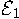
\includegraphics[]{E1.pdf}
	& 
	$\begin{aligned}[t] % placement: default is "center", options are "top" and "bottom"
	\vect{\kappa b}_{2i-1} 	& =  \frac{2}{L_{i-1}} \vect{u}_{2i-2} \times \vect{u}_{2i-1}\\[0.5em]
	\vect{\kappa b}_{2i+1} 	& =  \frac{2}{L_{i}} \vect{u}_{2i} \times \vect{u}_{2i+1} 
	\end{aligned}$
\end{tabularx}

% -------------------------------------------------------------------------------------
\subsubsection{Unit tangent vectors at ghost vertices}
% -------------------------------------------------------------------------------------

This definition of the curvature leads to a natural definition of the unit tangent vector at ghost vertex $\vect{x}_{2i-1}$ (resp. $\vect{x}_{2i+1}$), as the unit vector tangent to the osculating circle of the ($i-1$)\textit{th} segment (resp. $i$-\textit{th} segment) at that point. 

\begin{tabularx}{\textwidth}[t]{>{\centering\arraybackslash}m{0.48\textwidth} >{\centering\arraybackslash}X} % >{\centering\arraybackslash}
	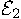
\includegraphics[]{E2.pdf}
	& 
	$\begin{aligned}[t] % placement: default is "center", options are "top" and "bottom"
	\vect{t}_{2i-1}	&=  \frac{l_{2i-1}}{L_{i-1}} \vect{u}_{2i-2}	+ 	\frac{l_{2i-2}}{L_{i-1}} \vect{u}_{2i-1} 	\\[0.5em]
	\vect{t}_{2i+1} 	&=  \frac{l_{2i+1}}{L_{i}} \vect{u}_{2i}		+ 	\frac{l_{2i}}{L_{i}} \vect{u}_{2i+1} 	
	\end{aligned}$
\end{tabularx}

% -------------------------------------------------------------------------------------
\subsubsection{Left/right unit tangent vectors at handle vertices}
% -------------------------------------------------------------------------------------

Equivalently, the definition of the osculating circles of the ($i-1$)\textit{th} and $i$-\textit{th} segments leads to a natural definition of the left ($\vect{t}_{2i}^-$) and right ($\vect{t}_{2i}^+$) unit tangent vectors at handle vertex $\vect{x}_{2i}$, for segments of uniform curvature. When both segments have the same curvature, left and right vectors agree.

\begin{tabularx}{\textwidth}[t]{>{\centering\arraybackslash}m{0.48\textwidth} >{\centering\arraybackslash}X} % >{\centering\arraybackslash}
	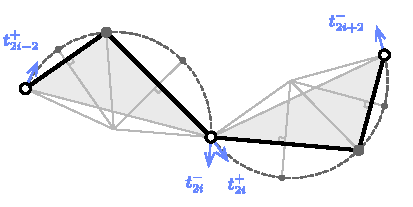
\includegraphics[]{E3.pdf}
	& 
	$\begin{aligned}[t] % placement: default is "center", options are "top" and "bottom"
	\vect{t}_{2i}^- 	&= 2 (\vect{t}_{2i-1} \cdot \vect{u}_{2i-1}) \vect{u}_{2i-1} - \vect{t}_{2i-1} \\[0.5em]
	\vect{t}_{2i}^+ 	&= 2 (\vect{t}_{2i+1} \cdot \vect{u}_{2i}) \vect{u}_{2i} - \vect{t}_{2i+1}
	\end{aligned}$
\end{tabularx}

% -------------------------------------------------------------------------------------
\subsubsection{Unit tangent vectors at handle vertices}
% -------------------------------------------------------------------------------------

The unit tangent vector $\vect{t}_{2i}$ -- that is the beam section normal -- at handle vertex $\vect{x}_{2i}$ is chosen to be the mean of the left and right unit tangent vectors at that vertex.\footnote{Consequently, this model assumes that the field of tangents along the centerline is continuous and is thus unable to model cases where the centerline is not at least $\mathcal{C}^1$. In such case the beam must be considered as two parts glued together.}

\begin{tabularx}{\textwidth}[t]{>{\centering\arraybackslash}m{0.48\textwidth} >{\centering\arraybackslash}X} % >{\centering\arraybackslash}
	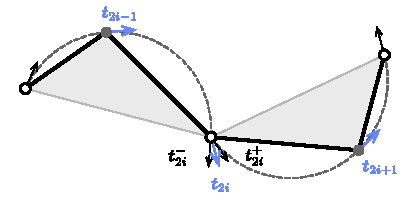
\includegraphics[]{E4.pdf}
	& 
	$\begin{aligned}[t] % placement: default is "center", options are "top" and "bottom"
	\vect{t}_{2i} 	&= \frac{\vect{t}_{2i}^- + \vect{t}_{2i}^+ }{\norm{\vect{t}_{2i}^- + \vect{t}_{2i}^+}}
	\end{aligned}$
\end{tabularx}

This way, the determination of the tangent vectors -- or equivalently the section normals -- in the static equilibrium configuration will be done in the flow of the dynamic relaxation process, without the need of introducing any additional degrees of freedom (for instance the usual Euler angles). The position of the vertices rules the orientation of the section normals.

% -------------------------------------------------------------------------------------
\subsubsection{Left/right bending moments at handle vertices}
% -------------------------------------------------------------------------------------

Given the unit tangent vector $\vect{t}_{2i}$, one can define the left ($\vect{\kappa}_{2i}^-$) and right ($\vect{\kappa}_{2i}^+$) curvatures at handle vertex $\vect{x}_{2i}$. The left curvature is initially evaluated from the left osculating circle, defined as the circle passing through $\vect{x}_{2i-1}$ and $\vect{x}_{2i}$ and tangent to $\vect{t}_{2i}$ at $\vect{x}_{2i}$. The right curvature is initially evaluated from the right osculating circle, defined as the circle passing through $\vect{x}_{2i}$ and $\vect{x}_{2i+1}$ and tangent to $\vect{t}_{2i}$ at $\vect{x}_{2i}$.\footnote{Remark that the centerline is now approximated with a biarc in the vicinity of $\vect{x}_{2i}$. This is the reason why this model is called the \textquote{biarc model}.}${}^,$\footnote{This model offers the ability to represent discontinuities in curvature -- thus in bending moment -- at handle vertices as the left and right curvatures does not necessarily agree. This is quite different from the classical 3-dof element \cite{Barnes1999, Adriaenssens1999, Douthe2006} which assumes that the curvature -- thus the bending moment -- is $\mathcal{C}^0$ and can be evaluated at every vertices from the circumscribed osculating circle.}

\begin{tabularx}{\textwidth}[t]{>{\centering\arraybackslash}m{0.48\textwidth} >{\centering\arraybackslash}X} % >{\centering\arraybackslash}
	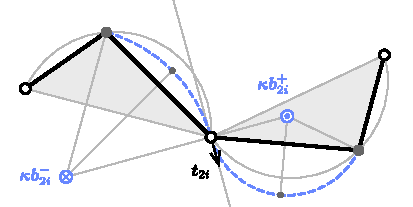
\includegraphics[]{E5.pdf}
	& 
	$\begin{aligned}[t] % placement: default is "center", options are "top" and "bottom"
	\vect{\kappa b}_{2i}^- &=  \frac{2}{l_{2i-1}} \vect{u}_{2i-1} \times \vect{t}_{2i}
	\\[0.5em]
	\vect{\kappa b}_{2i}^+ &=  \frac{2}{l_{2i}} \vect{t}_{2i} \times \vect{u}_{2i}
	\end{aligned}$
\end{tabularx}

However, this values need to be adjusted so that the static condition for rotational equilibrium ($\vect{M}^{ext}  + \vect{M}^+ - \vect{M}^- = 0$) is satisfied at all time. Then, this condition will be satisfied -- in particular -- at the end of the solving process. To achieve this goal, we first compute a realistic mean value ($\vect{M}_{2i}$) for the internal bending moment as :
\begin{equation}
		\vect{M}_{2i} 	=  \frac{1}{2} \mat{B}_{i-1}(\vect{\kappa b}_{2i}^- - \rconf{\vect{\kappa b}}_{2i}^-)
					+  \frac{1}{2} \mat{B}_{i}(\vect{\kappa b}_{2i}^+ - \rconf{\vect{\kappa b}}_{2i}^+)
\end{equation}
To enforce the jump discontinuity in bending moment ($\vect{M}^{ext} = \vect{M}^- - \vect{M}^+$) across the handle vertex, we define the left and right bending moments at $\vect{x}_{2i}$ as :
\begin{subequations}
	\begin{align}
		\vect{M}_{2i}^- 	&=  \vect{M}_{2i} + \frac{1}{2} \vect{M}_{2i}^{ext} 
		\\[0.5em]
		\vect{M}_{2i}^+ 	&=  \vect{M}_{2i} - \frac{1}{2} \vect{M}_{2i}^{ext} 
	\end{align}
\end{subequations}
Note that in the case where no external concentrated bending moment is applied to the handle vertex, the internal bending moment is continuous across the vertex.

% -------------------------------------------------------------------------------------
\subsubsection{Left/right curvatures at handle vertices}
% -------------------------------------------------------------------------------------

Finally, the left and right curvatures at handle vertex $\vect{x}_{2i}$ are computed back with the constitutive law :
\begin{subequations}
	\begin{align}
		\vect{\kappa b}_{2i}^-  &=  \mat{B}_{i-1}^{\;-1} \vect{M}_{2i}^- + \rconf{\vect{\kappa b}}_{2i}^- 
		\\[0.5em]
		\vect{\kappa b}_{2i}^+  &=  \mat{B}_{i}^{\;-1} \vect{M}_{2i}^+ + \rconf{\vect{\kappa b}}_{2i}^+ 
	\end{align}
\end{subequations}

% -------------------------------------------------------------------------------------
\subsubsection{Bending moment at ghost vertices}
% -------------------------------------------------------------------------------------

The internal bending moment at ghost vertices is simply given by the constitutive law as :
\begin{subequations}
	\begin{align}
		\vect{M}_{2i-1} &=  \mat{B}_{i-1}(\vect{\kappa b}_{2i-1} - \rconf{\vect{\kappa b}}_{2i-1})
		\\[0.5em]
		\vect{M}_{2i+1} &=  \mat{B}_{i}(\vect{\kappa b}_{2i+1} - \rconf{\vect{\kappa b}}_{2i+1})
	\end{align}
\end{subequations}

\subsection{Discret twisting moment}
% ==========================

We assume the twisting moment and the rate of twist to vary linearly over $]\vect{x}_{2i},  \vect{x}_{2i+2}[$.
Thus, the rate of twist at mid edge is given by :
\begin{equation}
	\tau_{i+1/2} = \frac{\Delta\theta_{i}}{l_i}
\end{equation}
And $\theta_{i+1} - \theta_{i}$ is the additional twisting angle between two frames with parallel transport.
\begin{equation}
	Q_{i+1/2} =  GJ(\tau_{i+1/2} - \rconf{\tau}_{i+1/2})
\end{equation}

\subsection{Discret axial force}

We assume the axial force and the axial strain to vary linearly over $]\vect{x}_{2i},  \vect{x}_{2i+2}[$.
Thus, the axial strain at mid edge is given by :
\begin{equation}
	\epsilon_{i+1/2} = \frac{l_{i}}{\rconf{l_i}} - 1
\end{equation}
\begin{equation}
	N_{i+1/2} =  ES\epsilon_{i+1/2}
\end{equation}

\subsection{Discret shear force}

Shear forces are computed from the second Kirchhoff law, considering that the inertial term is negligible.

\begin{equation}
	 \vect{F}_{i+1/2} = \vect{d}_{3, i+1/2} \times (\vect{M}_{i+1/2}^{'} + \vect{m}_{ext, i}) + Q_{i+1/2} \vect{\kappa b}_{i+1/2} - \tau_{i+1/2} \vect{M}_{i+1/2}
\end{equation}

\subsection{Interpolation}


\section{Conclusion}
Remind that the beam is subject to a distributed external force $\vect{f}_{ext}$ and a distributed external moment $\vect{m}_{ext}$.

We neglect rotational inertial effects on $\vect{d}_1$ et $\vect{d}_2$ in \eqref{eq:3_16_b} and \eqref{eq:3_16_c} which leads to the following shear force :
\begin{equation}
	\vect{F}^{\perp}(s) = \vect{d}_3 \times (\vect{M}' + \vect{\Omega} \times \vect{M} + \vect{m}_{ext})
\end{equation}
\begin{equation}
	\vect{F}^{\parallel}(s) = N \vect{d}_3
\end{equation}
\note{We may neglect as well the last term ($\tau \vect{M}$) and get back to the shear force obtained by the variational approach.} The total internal force acting on the beam is hence given by :
\begin{equation}
	\vect{F}(s) = \vect{N}(s) + \vect{T}(s)
\end{equation}
Sections are subject to the following rotational moment around the centerline :
\begin{equation}
	\begin{aligned}
	\vect{\Gamma}(s) = Q' + \vect{d}_3 \cdot ( \kappa\vect{b} \times \mat{M} + \vect{m}_{ext})
	\end{aligned}
\end{equation}

\clearpage



\clearpage
\bibliographystyle{alpha}
\bibliography{../library}
